\chapter*{Введение}

Язык Python на сегодняшний день является одним из самых популярных. 
Он прочно занимает лидирующие позиции на рынке и используется для решения таких
задач как высоконагруженные веб-сервисы (для этих целей используются 
такие фреймворки как Django и Flask), обработка больших данных и 
решение сложных инженерных задач (здесь часто 
используют такие библиотеки как numpy и scipy), а также для работы 
с графическими интерфейсами (например, читатель может ознакомиться с 
библиотеками tkinter и PyQT) и даже для взаимодействия с 
микроконтроллерами. Python удобен тем, что он кросс-платформенный, 
некомпилируемый и достаточно прост в изучении.

Данная книга ориентирована на читателя, который не имеет представления
о языке Python и хочет изучить основы алгоритмов. В основном эта книга 
предназначена для учеников старших классов, а также для взрослых читателей,
которые хотят получить базовое представление об основных алгоритмах 
и структурах данных.

Эта книга состоит из пяти частей. В первой части книги приводятся 
базовые понятия из математики. Во второй части описываются ключевые 
компоненты языка Python. Затем, в третей главе, приводится описание 
базовых структур данных, таких как массивы, стеки, очереди, деревья,
графы и т.д. В четвертой главе мы познакомим читателя с основными 
приёмами при решении алгоритмических задач. К примеру, тут мы расскажем
о так называемом методе \bf{разделяй и властвуй}, \bf{жадных алгоритмах},
и закончим книгу рассказом о \bf{динамическом программирование}.  
И наконец, в последней главе, мы предоставим читателю финальный проект - 
разработка утилиты для построчного сравнения файлов. 

\chapter{Математические основы}

Прежде чем мы сможем приступить к изучению алгоритмов нам необходимо ознакомиться
с основными математическими понятиями и приёмами. В данной главе мы также приведем
базовые понятия из теории вероятности. Часто такие знания являются необходимыми
при стохастическом анализе алгоритмов. Например, когда требуется найти среднее 
время выполнения алгоритма, а не оценивать верхнюю или нижнюю границу для сложности. 
Но начнем мы наше приключение с таких основ как системы счисления, 
функции и математическая индукция.

\section{Системы счисления}

В повседневной жизни мы используем числа для некоторого количественного
представления чего либо. И как правило мы используем десятичную систему 
счисления. Но существуют и другие системы: двоичная, восьмеричная, 
шестнадцатеричная, и т.д. Например, компьютеры обычно используют 
двоичную систему счисления, так как $0$ можно представить как отсутствие 
электрического заряда, а $1$ можно представить как его наличие. 
В программирование иногда бывает удобней работать с двоичной системой
счисления, чем с привычной для нас десятичной системой. Для того что бы 
эффективно работать в разных системах, нужно вооружиться методами перевода
из одной системы в другую. В данной главе мы рассмотрим, как это можно сделать.

Начнем мы с двоичной системой счисления. Например, число $19_{10}$ в десятичной
системе будет равно $10011_{2}$ в двоичной. Как мы этого достигли? Возьмем число 
$19$ и представим его как линейную комбинацию: $19=2 \cdot 9 + 1$ (заметим, что в качестве 
множителя взято число $2$: такой выбор связан с тем, что мы переводим в двоичную систему 
счисления). Запомним результат. Далее возьмем целую часть от деления, 
число $9$, и также представим его как линейную комбинацию: $9=2 \cdot 4 + 1$. 
Будем продолжить данную операцию до тех пор, пока целая часть 
от деления не станет равна нулю. Представим наш пример в 
табличном виде (смотрите Таблицу~\ref{tab:binary}).

\begin{table}
\centering
\begin{tabular}{c|c|c}
\hline
Делимое & Целая часть & Остаток от деления \\\hline
\cellcolor{lightblue}19 & \cellcolor{lightblue}9 & \cellcolor{blue}1 \\
\cellcolor{lightblue}9  & \cellcolor{lightblue}4 & \cellcolor{lightblue}1 \\
\cellcolor{lightblue}4  & \cellcolor{lightblue}2 & \cellcolor{lightblue}0 \\
\cellcolor{lightblue}2  & \cellcolor{lightblue}1 & \cellcolor{lightblue}0 \\
\cellcolor{lightblue}1  & \cellcolor{lightblue}0 & \cellcolor{red}1 \\
\hline
\end{tabular}
\caption{Пошаговое вычисление числа в двоичной системе счисления}
\label{tab:binary}
\end{table}

В таблице, красным цветом отмечен наиболее значимый бит, синим же 
цветом отмечен наименее значимый бит. Тогда если мы запишем значения
последней колонки начиная с наиболее значимого бита, мы получим 
желаемое представления числа $19_{10}$ в двоичной системе счисления. 

Обратное преобразование проще. Для этого нам необходимо вычислить сумму:
$\sum_{i=0}^n b_i2^i$, где $b_i$ - это $i$ый бит в двоичном представлении
числа. Используя данные из нашего примера, который мы описали выше, мы 
получим $1\cdot2^0+1\cdot2^1+0\cdot2^2+0\cdot2^3+1\cdot2^4 = 19_{10}$.

Теперь, когда мы знаем как преобразовывать в двоичную систему, мы можем записать
этот алгоритм на языке Python:

\begin{python}
def dec_to_bin(a):
	binary = "";
	while a != 0:
		binary = str(a % 2) + binary;
		a = (a - (a % 2))/2;
	return binary;

def bin_to_dec(binary):
	accumulator = 0;
	for i in range(0, len(binary)):
		accumulator += int(binary[len(binary) - i - 1]) * (1 << i);
	return accumulator;
\end{python}

В языке Python есть специальная функция для перевода в двоичную систему счисления - \texttt{bin}.
Заметим, что число в двоичной системе в Python представляется как бинарное число, начинающееся со 
специального префикса - $0b$.

Такой же подход можно использовать для перевода числа из десятичной системы, скажем, в 
шестнадцатеричную. Например, возьмём число $181_{10}$, которое будет равно $B5_{16}$. 
В шестнадцатеричной системе счисления, помимо чисел $0-9$, используются первые $6$ букв 
латинского алфавита, т.е., $A, B, C, D, E, F$ (легко заметить, что символ $A$ будет в численном 
представление равен $10$, а символ $F$ - $15$). Таким образом, чтобы перевести число $B5_{16}$ из
шестнадцатеричной системы обратно в десятичную нужно вычислить сумму $\sum_{i=0}^{n} h_i \cdot 16^i$,
где $h_i$ - это численное представление символа в шестнадцатеричной системе счисления.
Для удобства Python поддерживает специальную функцию \texttt{hex}, которая может перевести 
число из десятичной системы счисления в шестнадцатеричную. По условию все числа в шестнадцатеричной 
системе счисления начинаются с префикса \texttt{0x}.

\section{Функции}

В математике функцией называется зависимость одной величины от другой. В любой функции,
если это функция одной переменной, есть независимая и зависимая переменные. Например, в функции
$y=2^x$, $y$ - это зависимая переменная, а $x$ - это независимая переменная, т.е., при изменении
$x$, соответствующим образом будет меняться и $y$. 

В рамках данной книги наибольший интерес представляют несколько видов функций, а именно: 
показательные, логарифмические, полиномиальные. Все эти функции ведут себя по разному, но
часто при анализе алгоритмической сложности нужно иметь представление о скорости роста функции.
Например, на Графике~\ref{fig:functions} мы наглядно приводим скорости роста самых основных 
функций (так как обычно при анализе алгоритмов переменная величина - это размер входных данных, 
то все значения на оси $X$ являются положительными целыми числами).

\begin{figure}[h!]
\centering
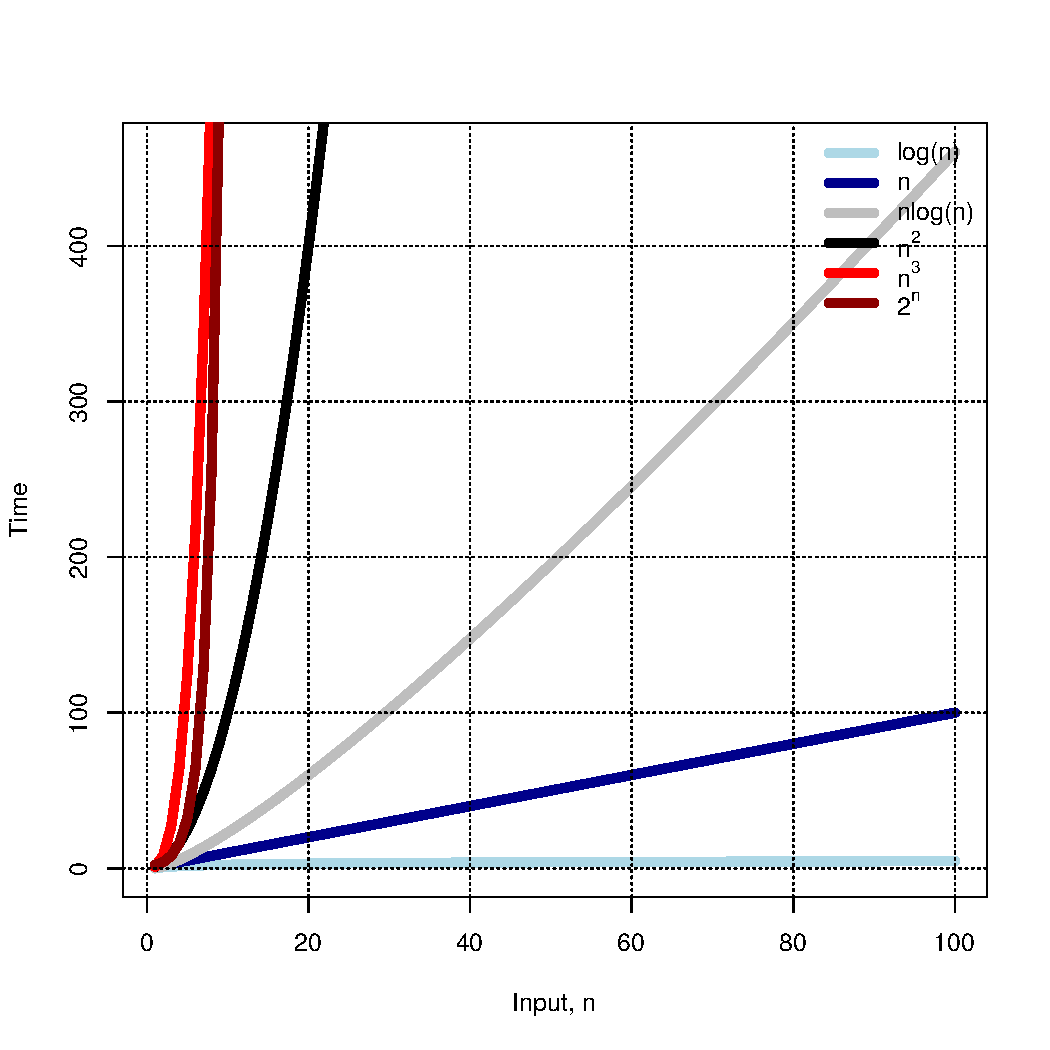
\includegraphics[width=0.6\textwidth]{graphics/functions.pdf}
\caption{Скорость роста различных функций}
\label{fig:functions}
\end{figure}

Показательные функции имеют вид $y=a^n$ (обычно за $n$ берется размер входных данных, т.е., 
$n$ - это переменная величина). Перечислим основные свойства показательных функций. 

\begin{definition}
Если основание показательной функции $0<a<1$, то функция монотонно убывает, если же $a>1$,
то функция монотонно возрастает.
\end{definition}

\begin{definition}
Если основания показательных функций равны, то $a^na^m=a^{n+m}$.
\end{definition}
\begin{definition}
Если основания показательных функций равны, то $\frac{a^n}{a^m}=a^{n-m}$.
\end{definition}
\begin{definition}
Пусть $y=a^n$, тогда $a^n+a^n=2a^n$. Или более общий вид $\sum_{i=1}^{k}a^n=ka^n$.
\end{definition}
\begin{definition}
Пусть $y=a^n$, тогда $y^m=a^{nm}$.
\end{definition}
Логарифмическая функция представляется в виде $y=\log_a(n)$. Обратная 
этой функции - это показательная функция, которую мы уже рассмотрели 
($a^y=n)$. Также как и предыдущий класс функций, логарифмы часто встречаются в 
анализе алгоритмов. Рассмотрим свойства этих функций. 

\begin{theorem}
Пусть дана логарифмическая функция $y=\log_an^b$, тогда $y=b\log_an$.
\end{theorem}
Так как $y=\log_an^b$, то $a^y=n^b$. Но если мы возведём обе стороны уравнения
в степень $1/b$, то получим $a^{y/b}=n^{b/b}=n$. Но по определению логарифма
мы имеем $\frac{y}{b}=\log_an$. Тогда помножив обе части уравнения на $b$
получим $y=b\log_an$, что и требовалось доказать.

\begin{theorem}
Если $y=\log_a(n)$, то $a^{\log_a(n)}=n$.
\end{theorem}
Так как $a^{\log_a(n)}=a^y$, а по определению логарифма $a^y=n$, 
то $a^{\log_a(n)}=n$. Что и требовалось доказать.

\begin{theorem} 
Пусть дана логарифмическая функция $\log_an$, тогда 
$\log_cn=\frac{\log_cn}{\log_ca}$.
\end{theorem}

Так как $y=\log_an$, то $a^y=n$. И пусть $z=\log_cn$, $c^z=n$. Тогда,
$a^y=c^z$. Прологарифмируем обе стороны уравнения,
тогда $y\log_aa=z\log_ac$, откуда следует $z=\log_cn=\frac{\log_an}{\log_ac}$.
Что и требовалось доказать.

\begin{theorem}
$\log_a(nm)=\log_an+\log_am$
\end{theorem}
$\log_a(nm)=\log_a(a^{\log_a(n)}a^{\log_a(m)})=\log_aa^{\log_a(n)+\log_a(m)}=\log_a(n)+\log_a(m)$.
Что и требовалось доказать.

\begin{theorem}
$\log_a\frac{n}{m}=\log_an-\log_am$
\end{theorem}
$\log_a(n/m)=\log_a(a^{\log_a(n)}/a^{\log_a(m)})=\log_aa^{\log_a(n)-\log_a(m)}=\log_a(n)-\log_a(m)$
Что и требовалось доказать.

Степенные функции $y=n^a$ также часто встречаются в анализе алгоритмов. Обычно, $n$ - это
переменная величина (размер входных данных), а $a \in \mathbb{N}$. Как мы увидим дальше,
обычно сложность алгоритмов со вложенными циклами можно представить именно этими функциями.

\section{Основные сведения о рядах}

Обширный обзор рядов и способов их анализа можно 
найти в~\cite{kudryavcev:math, stewart:calculus}. В данном же разделе 
приведем несколько сведений об основных свойствах рядов и 
как их можно анализировать (в основном мы заинтересованы в рядах с
конечным числом членов, так как они чаще встречаются на практике). 

Рядом называется последовательность чисел, где каждый член отличается от предыдущего 
на некоторую величину (бывают конечно и знакочередующиеся ряды, но
здесь мы такие не будем рассматривать). Например, ряд $0, 5, 10, 15, \ldots$ является 
арифметической прогрессией, в которой каждый член больше предыдущего на $5$. 
Еще один часто встречающийся ряд - это геометрическая прогрессия. 
Например, $1, 2, 4, 8, 16, 32, \ldots$ - это геометрическая 
последовательность, в которой $i$-ый член ряда можно найти, 
применив формулу $a_i = qa_{i-1} = q^{i-1}a_{1}$, где $q=2$, а $a_1 = 1$. В данном разделе
же приведем несколько примеров того, как можно анализировать суммы этих 
и некоторых других рядов (в основном нас интересуют ряды с конечным числом членов).

Например, пусть нам необходимо найти сумму следующего ряда:

$$S=\sum_{i=1}^{n}i = 1 + 2 + 3 + 4 + \ldots + n$$

Простой способ анализа, заключается в сложение первого и последнего членов ряда, и далее 
второго и предпоследнего членов, и т.д (здесь мы предполагаем, что количество членов 
является чётным числом). Тогда, заметив, что сумма таких пар равна $n+1$,
а количество пар равно $n/2$, можно предположить, что сумма ряда равна $\frac{n(n+1)}{2}$.
Если же $n$ - нечётное число, тогда можно доказать это утверждение, воспользовавшись методом немецкого 
математика Карла Гаусса, который он вывел в детстве. Возьмём $S+S=2S$. Тогда,
складывая первый и последний члены двух сумм получим 
$$2S=(1+n) + (n - 1 + 2) + \ldots + (1 + n) = (n+1)n$$
Очевидно, что искомая сумма равна $S=\frac{n(n+1)}{2}$.

Рассмотрим более общий пример. Пусть мы хотим вычислить сумму ряда $i^k$, где $k \ge 1$.
Но прежде, представим выражение $(a+b)^k$ в виде суммы. И так 
$$(a+b)^k = C^0_k a^kb^0+C^1_ka^{(k-1)}b^1 + ... + C^k_ka^0b^k$$
где $C^m_k = \frac{k!}{(k-m)!m!}$ - это сочетание.
Мы еще вернемся к этой формуле, когда будем рассказывать про правила вычисления
вероятностей, а пока отметим, что в формуле, которую мы определили только что $k!$ - это 
факториал, который вычисляется как $k! = 1\cdot2\cdot3\ldots k$. Причем $0!=1$.
Но вернемся к нашему разговору о вычислении суммы ряда. Возьмем для
примера $(i-1)^2 = i^2 - 2i + 1$.
Перенесём $i^2$ влево, домножим на $-1$ обе части уравнения и просуммируем:
$$\sum_{i=1}^n (i^2 - (i-1)^2) = \sum_{i=1}^n (2i - 1)$$
Заметим, что левая часть схлопывается и получается, что сумма 
равна $n^2$. В правой же части получаем $2S-n$, где $S$ - это искомая сумма.
Теперь, если мы решим уравнение для $S$, то получим
$S = \frac{n^2+n}{2} = \frac{n(n+1)}{2}$.
Такой же математический приём можно применить и к другим суммам, например $\sum_{i=1}^n i^2$.
Для этого разложим выражение 
$$(i-1)^3 = \\ 
C_3^0(-1)^0i^3+C_3^1(-1)^1i^2 + C_3^2(-1)^2i + C^3_3(-1)^3i^0 = \\
i^3-3i^2+3i-1$$
Аналогично предыдущему примеру, перенесем $i^3$ влево, домножим на $-1$ и
просуммируем обе части уравнения. Тогда получим:
$$\sum_{i=1}^n (i^3-(i-1)^3) = \sum_{i=1}^n(3i^2-3i+1)$$
Левая часть схлопывается и становится равной $n^3$, правую же часть можно представить как
$3S-\frac{3n(n+1)}{2} + n$. После перестановки членов в левой и правой частях, получаем:
\begin{equation*}
\begin{multlined}
S=\frac{2n^3 - 2n + 3n(n+1)}{6} = \frac{2n(n^2 - 1) + 3n(n + 1)}{6} = \\
\frac{2n(n - 1)(n+1) + 3n(n+1)}{6} = \frac{(2n(n - 1) + 3n)(n+1)}{6} = \\
\frac{(2n^2 + n)(n+1)}{6} = \frac{n(2n + 1)(n+1)}{6}
\end{multlined}
\end{equation*}
Данный метод хорош тем, что его можно применить для нахождения суммы любого ряда вида $i^k$, при условии, что $k \ge 1$

Ещё один часто встречающийся ряд - это геометрическая прогрессия. Сумму такого ряда можно представить
как:

$$S = \sum_{i=0}^{n}aq^i = a(1 + q + q^2 + q^3 + \ldots + q^n)$$

Простой способ нахождения суммы этого ряда заключается перемножение $S$ 
на $q$ и решение следующего уравнения $S - qS = a(1 - q^{n+1})$ (заметим, правая часть
получилась путём вычитания $qS$ из $S$). Тогда, сумма ряда равна $S=\frac{a(1-q^{n+1})}{1-q}$.

Иногда найти сумму ряда бывает сложно и проще дать аппроксимацию.
Например, рассмотрим гармонический ряд $1, \frac{1}{2}, \frac{1}{3}, \ldots,\frac{1}{n}$. 
Тогда сумма этого ряда тогда будет равна $$H_n = \sum_{i=1}^n\frac{1}{i} \approx \int_1^n\frac{dx}{x} = \ln(n)$$

\section{Множества}

В математике множеством называется совокупность объектов любого типа~\cite{turner:probability}.
Например, множеством является набор букв латинского алфавита - $\{a, b, c, \ldots, z\}$, или множества 
все целых чисел - $x \in \mathbb{Z}$. Обычно, для обозначения множеств, используют прописные буквы 
латинского алфавита, а элементы заключают в фигурные скобки. Например, $A=\{a, b, c\}$ или 
$X=\{x: x > 10\}$. Принадлежность элемента $x$ к множеству обычно обозначают символом $\in$.
Приведём несколько определений.

\begin{definition}
Пустое множество - это такое множество, которое не содержит элементы. Обозначается
такое множество как $\emptyset$. 
\end{definition}

\begin{definition}
$A$ является подмножеством множества $B$, если все элементы
множества $A$ также являются элементами множества $B$. Обозначается это свойство следующим образом:
$A \subset B$. 
\end{definition}

%И наконец, дадим определение универсальному множеству.

\begin{definition}

Универсальное множество - это такое множество, которое содержит все 
элементы. Обычно такое множество обозначается как $\Omega$. Например, пусть $\Omega$ - множество 
всех возможных значений игральной кости, т.е., $\Omega = \{1, 2, 3, 4, 5, 6\}$. 
\end{definition}

\begin{definition}
Если элементы некоторого множества $A'$ принадлежат универсальному множеству, но не принадлежат
множеству $A$, то такое множество называется дополнением множества $A$: 
$A' = \{x: x \in \Omega \wedge x \notin A\}$.
\end{definition}

Над множествами, как и над числами, можно производить операции. Таким образом, далее мы рассмотрим 
операции сложения (или объединения), пересечения и вычитания множеств. А после приведем (без доказательств) основные свойства множеств.

\begin{definition}
Объединением множества $A$ и $B$ называется такое множество, которое 
содержит элементы, принадлежащие или множеству $A$, или множеству $B$. 
Математически эта операция записывается следующим образом:
$A \cup B = \{x: x \in A \vee x \in B\}$.
\end{definition}

\begin{definition}
Пересечением множества $A$ и $B$ называется такое множество, которое
содержит элементы, принадлежащие одновременно и множеству $A$, и 
множеству $B$. Математически эта операция записывается следующим образом:
$A \cap B = \{x: x \in A \wedge x \in B\}$.
\end{definition}

\begin{definition}
Разностью множеств $A$ и $B$ называется такое множество, которое
содержит элементы множества $A$, но не содержит элементы принадлежащие  
множеству $B$. Математически эта операция записывается следующим образом:
$A \setminus B = \{x: x \in A \wedge x \notin B\}$.
\end{definition}

Мы еще вернемся к обсуждению операций над множествами, когда будем рассматривать 
работу с множествами в языке Python. А пока, рассмотрим основные свойства 
множеств, которые часто встречаются на практике (смотрите 
Таблицу~\ref{tab:set:properties}).

\begin{table}[ht!]
\centering
\small
\begin{tabular}{|c|c|c|}
\hline
Идемпонентный закон       & $A \cup A = A$            & $A \cap A = A$                 \\\hline
Закон тождества           & $A \cup \emptyset = A$    & $A \cap \emptyset = \emptyset$ \\
                          & $A \cup \Omega = \Omega$  & $A \cap \Omega = A$            \\\hline
Закон дополнения          & $A \cup A' = \Omega$ & $A \cap A' = \emptyset$ \\\hline
Закон коммутативности     & $A \cup B = B \cup A$     & $A \cap B = B \cap A$ \\\hline
Закон ассоциативности     & $(A \cup B) \cup C = $ & $(A \cap B) \cap C =$ \\
                          & $A \cup (B \cup C)$    & $A \cap (B \cap C)$ \\\hline
Закон дистрибутивности    & $A \cup (B \cap C) = $ & $A \cap (B \cup C) = $ \\
                          & $(A \cup C) \cap (A \cup B)$ & $(A \cap C) \cup (A \cap B)$ \\\hline
Закон Де Моргана          & $(A \cup B)'= A' \cap B'$ & $(A \cap B)'=A' \cup B'$ \\\hline
\end{tabular}
\caption{Основные свойства множеств}
\label{tab:set:properties}
\end{table}

\section{Алгоритмическая сложность}
\label{sec:complexity}

Алгоритм - это некая последовательность инструкций компьютера, которые необходимо воспроизвести, 
чтобы решить поставленную задачу. Как только алгоритм составлен и написан в виде инструкций языка,
например такого как Python, его желательно проанализировать, чтобы знать его производительность.
Сложность алгоритма обычно выражают как функцию $T(n)$, где $n$ - это длина входных данных. 

Обычно, вычислительную сложность записывают используя правила большого $O$ (или $Big\ O$, как эти правила 
принято называть в иностранной литературе). Введем несколько определений. Пусть вычислительная 
сложность задана функцией $T(n)$, тогда~\cite{weiss:dsaa}:

\begin{definition}
$T(n) = O(f(n))$ если есть некая константа $c > 0$ и функция $f(n)$ такая, что $T(n) \le c \cdot f(n)$, где $n>n_0$.
\end{definition}

\begin{definition}
$T(n) = \Omega(g(n))$ если есть некая константа $c > 0$ и функция $g(n)$ такая, что $T(n) \ge c \cdot g(n)$, где $n>n_0$.
\end{definition}

\begin{definition}
$T(n) = \Theta(h(n))$ если $T(n) = O(h(n))$ и $T(n) = \Omega(h(n))$.
\end{definition}

Иными словами, с помощью $O$ описывают верхнюю границу для сложности (памяти или вычислений), $\Omega$ используется для определения нижней границы, а используя $\Theta$ можно определить более строгую 
границу. Например, если $T(n) = 10n$, то конечно можно определить $T(n) = O(n^2)$ или даже $T(n) = O(n^3)$,
но более точным определением будет $T(n) = \Theta(n)$, так как можно выбрать в виде функции $h(n) = n$, а две константы выбрать как $c_1=1$, а $c_2=100$. Но так как не всегда можно дать точную оценку для 
сложности алгоритма, то обычно используют оценку $O$, так как её часто бывает проще найти.

Рассмотрим несколько примеров того, как можно анализировать циклы. Если в алгоритме 
всего один цикл (без вложенных циклов), тогда задача сводиться к подсчёту операций 
выполняемых в теле цикла. Но так как цикл выполняется $n$ раз (где $n$ - это размер входных 
данных), то нахождение общего времени выполнения алгоритма можно представить в виде простой суммы.
Например, в задаче нахождения максимальной суммы в последовательности (алгоритм приведен ниже),
на каждой итерации алгоритма выполняется $c=6$ инструкций. Тогда, общее количество операций 
$\sum_{i=1}^n c = nc$. Сложность же данного алгоритма можно оценить как $\Theta(n)$.

\begin{python}
def maximum_subsequence(a):
	max_sum = 0;
	current_sum = 0;
	start = 0;
	current_start = 0;
	end = 0;
	for i in range(0, len(a)):
		current_sum += a[i];
		if current_sum > max_sum:
			max_sum = current_sum;
			end = i + 1;
			start = current_start;
		if current_sum < 0:
			current_sum = 0;
			if i + 1 < len(a):
				current_start = i + 1;
	return (max_sum, a[start:end]);
\end{python}

Если же есть вложенные циклы, как например в задаче сортировки массива пузырьком, 
который мы приводим ниже, то сначала нужно проанализировать сложность 
вложенного цикла и только потом приступать к анализу внешнего цикла. Так, в примере,
который мы приводим ниже вложенный цикл выполняет $4(n-i)$ операций 
(здесь анализ аналогичен тому, который мы его 
провели в предыдущем примере). Тогда общая сложность
алгоритма может быть представлена в виде следующей суммы 
$\sum_{i=1}^n4(n-i) = \sum_{i=1}^n4n - \sum_{i=1}^n4i = 4n^2 - 4\frac{n(n+1)}{2} = 4n^2-2n^2 - 2n=2n^2 - 2n$.
Следовательно, сложность алгоритма может быть оценена как $O(n^2)$.

\begin{python}
def bubble_sort(a):
	for i in range(0, len(a)):
		for j in range(i, len(a)):
			if a[i] > a[j]:
				s = a[i];
				a[i] = a[j];
				a[j] = s;
	return a;
\end{python}

Приведём еще один известный, но неэффективный алгоритм сортировки - сортировка вставками. Сложность
данного алгоритма такая же, как и у сортировки пузырьком - в худшем случае алгоритму требуется $O(n^2)$
вычислений. Но в отличии от предыдущего алгоритма, в лучшем случае этому методу требуется $\Theta(n)$ вычислений
(например если массив уже отсортирован).

\begin{python}
def insertion_sort(a):
	for i in range(1, len(a)):
		j = i - 1;
		key = a[i];
		while True:
			if a[j] > key:
				a[j + 1] = a[j];				
				a[j] = key;
				j -= 1;
			if j <= 0 or a[j] <= key:
				break;
	return a;
\end{python}


Аналогичный прием можно применять и для алгоритмов с большим числом вложенных
циклов.

\section{Индукция и прочие приёмы доказательств}

Математическая индукция - это метод, который позволяет доказать истинность утверждения
путем перехода от частного к общему. Обычно в математической индукции на первом шаге
доказывается, что утверждение верно для некоторого значения (обычно небольшого). Далее,
предполагается, что выражение истинно для некоторого большого значения $n$. И наконец, 
доказывается, что выражение правдиво для $n+1$.

Приведем пример. Пусть мы предполагаем, что $\sum_{i=1}^n i=\frac{n(n+1)}{2}$. Убедимся, что утверждение
истинно для $n \in \{1, 2, 3\}$. Что безусловно очевидно, если мы вычислим сумму используя левое и правое выражения.
Далее предположим, что выражение истинно для некоторого $n$. И наконец, докажем, что при $n+1$, сумма равна $\frac{(n+1)(n+2)}{2}$. Действительно, $$\sum_{i=1}^{n+1} i=\frac{n(n+1)}{2} + n+1 = \frac{n(n+1) + 2(n+1)}{2} = \frac{(n+1)(n+2)}{2}$$ Что и требовалось доказать.

Помимо индукции существуют и другие подходы к доказательству математических свойств. Например,
доказать утверждение можно \bf{противоречием} или же контрпримером. 

Приведём пример доказательства контрпримером. Докажем что, $2^n<n!$, где $n>4$. Предположим обратное 
$2^n>n!$, но взяв $n=5$ мы получаем $32<120$, что противоречит утверждению.

\section{Рекурсия}

В программирование рекурсивная функция - это такая функция, которая вызывает сама себя. При 
каждом вызове размер входных данных должен уменьшаться и рекурсивные вызовы
прекращаются (обычно) когда размер входных данных равен единице. Примером рекурсии 
может служить функция вычисления наибольшего общего делителя. Мы еще столкнемся с ней,
когда будем описывать бинарные операторы. Сейчас же мы приведем ее как пример 
того, как рекурсия выглядит в программировании. Вслед за этим мы рассмотрим как
можно анализировать рекурсии (в математическом смысле).

\begin{python}
def gcd(a, b):
 if b == 0:
  return a;
 return gcd(b, a % b);
\end{python}

Для того, чтобы понять как изменяется размер входных данных в описанном выше алгоритме, 
приведём следующую теорему.

\begin{theorem}
Для любых целых чисел $a$ и $b$ (где $a>b$) справедливо неравенство: $a\ mod\ b < \frac{a}{2}$
\end{theorem}

Рассмотрим два случая: (i) это когда $b$ входит в $a$ точно один раз, т.е., $a = b + r$
(ii) это когда $b$ входит в $a$ несколько раз, т.е., $a = bq + r$.
Для случая (i) мы имеем $r < b$, но так как $b$ входит в a один раз, очевидно, что
$b > a/2$ (иначе $q > 1$) и соответственно $r < a/2$; (ii) так как $b$ входит в $a$ несколько раз, то $q \ge 2$,
соответственно $a > qb$ (иначе $r$ было бы равно $0$) из чего следует, 
что $b < a/q \le a/2$. Но так как $b > r$ (всегда), то и $r < a/2$. Что и требовалось доказать.

В рекурсии, время необходимое для вычисления обычно выражается как $T(n)$, где $n$ - это
размер входных данных. Используя нашу теорему, мы можем составить следующее рекуррентное соотношение (
мы полагаем, что при каждом рекурсивном вызове $b$ уменьшается как минимум вдвое).

$$T(n) = T(n/2) + 1 = 
	 T(n/4) + 2 = 
         T(n/8) + 3 = 
	 T(n/2^i) + i
$$

Зная, что когда размер входных данных равен единице рекурсия прекращается, то мы можем вычислить
$i$ через $n/2^i=1$ (обратите внимание, что это предположение следует из $T(n/2^i)=T(1)$). 
Далее мы имеем $n=2^i$. Прологарифмировав обе части уравнения, получаем
$i=\log_2(n)$, тогда выкладки, изложенные выше, дают нам возможность предположить, что сложность
алгоритма нахождения наибольшего общего делителя будет $O(\log(n))$.

Стоит отметить, как мы вывели $T(n)$: зная, что при каждом вызове, размер входных данных уменьшается в
двое, то $T(n/2) = T(n/2\cdot1/2) + 1 = T(n/4)+1$. Подставляя данное значение в выражение 
$T(n) = T(n/2) + 1$, мы можем вычислить $T(n)$ через $T(n/4)$ таким образом, получая $T(n)=T(n/4)+2$.
Продолжая этот ход мыслей, мы получаем выражение $T(n)=T(n/2^i) + i$.

\section{Булева логика}

Булева логика - это раздел математики, изучающий логические высказывания и операции над ними.
Логические высказывания могут быть простыми и составными. Например, составными высказываниями
являются такие высказывания, в которых есть несколько простых логических высказываний объединённых
логическими операциями. В данном разделе мы коротко ознакомимся с такими логическими операциями как:
конъюнкция (или операция И), дизъюнкция (или логическая операция ИЛИ), импликация (или следование),
равносильность (или эквивалентность), а также строгая дизъюнкция. Рассмотрим простейшие примеры 
булевой алгебры, а потом рассмотрим её основные свойства.

Начнем мы наше обсуждение с такой операции как отрицание. Пусть дано высказывание,
которое может принимать значения $1$ и $0$ (или же истина и ложь). 
Тогда справедливы утверждения описанные в Таблице~\ref{tab:negation}.

\begin{table}[!h]
\centering
\begin{tabular}{|c|c|}
\hline
$A$ & $\neg A$ \\\hline
0   & 1 \\\hline
1   & 0 \\\hline
\end{tabular}
\caption{Логическая операция отрицания}
\label{tab:negation}
\end{table}

Результат конъюнкции, или же иными словами операции логического И, становится истинным тогда, когда оба 
выражения истины, и становиться ложью, тогда, когда хотя бы одно выражение ложь. Составим следующую таблицу
истинности (смотрите Таблицу~\ref{tab:conjuction}). 

\begin{table}[!h]
\centering
\begin{tabular}{|c|c|c|}
\hline
$A$ & $B$ & $A \wedge B$ \\\hline
0   &  0  &  0 \\\hline
1   &  0  &  0 \\\hline
0   &  1  &  0 \\\hline
1   &  1  &  1 \\\hline
\end{tabular}
\caption{Конъюнкция}
\label{tab:conjuction}
\end{table}

Дизъюнкция - это логическая операция, результат которой будет истиной только тогда, когда
хотя бы одно выражение является истиной. Запишем эту операцию в виде таблицы истинности (смотрите
Таблицу~\ref{tab:disjunction}).

\begin{table}[!h]
\centering
\begin{tabular}{|c|c|c|}
\hline
$A$ & $B$ & $A \vee B$ \\\hline
0   &  0  &  0 \\\hline
1   &  0  &  1 \\\hline
0   &  1  &  1 \\\hline
1   &  1  &  1 \\\hline
\end{tabular}
\caption{Дизъюнкция}
\label{tab:disjunction}
\end{table}

Импликация - это логическая операция, которая гласит: из лжи может следовать что угодно, а
из истины только истина. В Таблице~\ref{tab:implication} представим результаты этой логической 
операции. Заметим, что импликацию можно заменить следующим сложным логическим 
высказыванием: $(\lnot A \vee B)$.

\begin{table}[!h]
\centering
\begin{tabular}{|c|c|c|}
\hline
$A$ & $B$ & $A \rightarrow B$ \\\hline
0   &  0  &  1 \\\hline
0   &  1  &  1 \\\hline
1   &  0  &  0 \\\hline
1   &  1  &  1 \\\hline
\end{tabular}
\caption{Импликация}
\label{tab:implication}
\end{table}

Операция эквивалентности гласит, что если оба логических высказывания либо истина либо ложь, тогда
результат всегда истина (смотрите Таблицу~\ref{tab:equivalence}). Заметим, что операцию эквивалентности
можно заменить следующим сложным логическим высказыванием: $(\lnot A \vee B) \wedge (A \vee \lnot B)$.

\begin{table}[!ht]
\centering
\begin{tabular}{|c|c|c|}
\hline
$A$ & $B$ & $A \leftrightarrow B$ \\\hline
0   &  0  &  1 \\\hline
0   &  1  &  0 \\\hline
1   &  0  &  0 \\\hline
1   &  1  &  1 \\\hline
\end{tabular}
\caption{Эквивалентность}
\label{tab:equivalence}
\end{table}

И наконец, приведем таблицу (смотрите Таблицу~\ref{tab:xor}) 
истинности для операции строгой дизъюнкции (в языках 
программирования такую операцию часто называют еще исключающее ИЛИ). 
Исключающее или можно заменить следующим сложным логическим
высказыванием: $(\lnot A \wedge B) \vee (A \wedge \lnot B)$. 

\begin{table}[!h]
\centering
\begin{tabular}{|c|c|c|}
\hline
$A$ & $B$ & $A \oplus B$ \\\hline
0   &  0  &  0 \\\hline
0   &  1  &  1 \\\hline
1   &  0  &  1 \\\hline
1   &  1  &  0 \\\hline
\end{tabular}
\caption{Строгая дизъюнкция}
\label{tab:xor}
\end{table}

\begin{table}[!ht]
\centering
\begin{tabular}{|c|c|c|}
\hline
Закон коммутативности     & $A \vee B = B \vee A$ \\
                          & $A \wedge B = B \wedge A$ \\\hline
Закон ассоциативности     & $(A \vee B) \vee C = A \vee (B \vee C)$ \\
                          & $(A \wedge B) \wedge C = A \wedge (B \wedge C)$ \\\hline
Закон дистрибутивности    & $A \vee (B \wedge C) = (A \vee B) \wedge (A \vee C)$ \\
                          & $A \wedge (B \vee C) = (A \wedge B) \vee (A \wedge C)$ \\\hline
Закон непротиворечия      & $A \wedge \lnot A = 0$ \\\hline
Закон исключения третьего & $A \vee \lnot A = 1$ \\\hline
Закон двойного отрицания  & $\lnot(\lnot A) = A$ \\\hline
Законы Де Моргана         & $\lnot (A \vee B) = \lnot A \wedge \lnot B$ \\
                          & $\lnot (A \wedge B) = \lnot A \vee \lnot B$ \\\hline
Закон рефлексии           & $A \vee A = A$ \\
                          & $A \wedge A = A$ \\\hline
Законы поглощения         & $A \vee (A \wedge B) = A$ \\
                          & $A \wedge (A \vee B) = A$ \\
                          & $A \vee (\lnot A \wedge B) = A \vee B$ \\\hline
Свойства логических констант & $A \vee 1 = 1$ \\
                             & $A \wedge 1 = A$ \\
                             & $A \vee 0 = A$ \\
                             & $A \wedge 0 = 0$ \\\hline
\end{tabular}
\caption{Основные свойства булевой алгебры}
\label{tab:logic:properties}
\end{table}

Заметим, что все эти логические операции часто используются в языках 
программирования, когда составляются ветвления. Мы еще вернемся 
к обсуждению составления логических выражений, когда будем обсуждать
ветвления и логические операторы в языке Python. А пока в 
Таблице~\ref{tab:logic:properties} приведём основные свойства булевой
алгебры.

\section{Базовые сведения из теории вероятности}

В данном разделе приведём несколько основных сведений о теории вероятности. 
Более подробный курс можно пройти, прочитав~\cite{turner:probability, kremer:probability}.

\subsection{Классическое определение вероятности}

Событием в теории вероятности называется какой либо исход, 
результат испытания. Например, при однократном бросании 
монеты возможными исходами могут быть выпадение орла или 
решки. События обычно обозначаются заглавными 
латинскими буквами. Таким образом, вероятность выпадения решки (появление 
события $A$), при однократном бросании монеты, можно записать в виде 
$P(A) = \frac{1}{2}$. Обратное же событие - выпадение орла, 
можно записать как $P(\bar{A})=1-P(A)$. В данном случае 
выпадение орла и решки имеют одинаковые вероятности и поэтому называются 
равновозможными. Если же события неравновероятные, то обычно 
задают закон распределения вероятностей, который каждому 
событию сопоставляет соответствующую вероятность. Мы еще вернёмся к
обсуждению законов распределения вероятностей чуть позже. А пока отметим, что 
в классической теории вероятности, вероятность наступления события $A$
может быть вычислена как $P(A)=\frac{m}{n}$, где $m$ - это 
количество исходов благоприятствующих событию, а $n$ - это количество
всех исходов. Отметим ещё один важный момент. Если события 
являются единственно возможными (т.е., в результате испытания
должно произойти хотя бы одно событие) и несовместными (т.е., ни одно 
событие не влечет за собой появление любого другого события), то такие события 
образуют полную группу. Например, в нашем примере с бросанием
монеты, события (выпадение орла или решки) образуют полную группу.

Отметим основные свойства вероятностей. Так например, вероятность 
наступления события заключена между нулём и единицей, т.е., $0 \le P(A) \le 1$.
Вероятность наступления достоверного события (событие, которое наступает
всегда) будет равно единице, т.е., $P(\Omega) = 1$. Вероятность же 
события, которое никогда не наступит (т.е., невозможное событие)
равно нулю, или $P(\emptyset)=0$. Сумма вероятностей единственно возможных и 
несовместных исходов равна единице, т.е., $\sum_{i=1}^nP(A_i)=1$.

Вернёмся к обсуждению способов вычисления вероятностей. Обычно, 
чтобы вычислить количество благоприятных и общее количество 
исходов пользуются комбинаторикой - разделом математики, 
который в том числе предлагает инструменты необходимые для 
подсчета количества исходов. 

%Пусть даны элементы $A_i$ (где $i \in \{1, \ldots, k\}$) некого конечного множества. 
Определим \textbf{правило сложения} следующим образом:
Пусть элемент $A_i$ может быть выбран $n_i$ способами (например,
в корзине имеется $10$ красных шаров, тогда $A_i$ - это красный шар, а $n_i=10$
- это количество таких шаров). Тогда выбор одного элемента 
(или $A_1$, или $A_2$, и т.д.) можно произвести 
$n = \sum_{i=1}^k n_i$ способами.

Например, пусть в урне имеется $100$ шаров: $30$ белых шаров, $10$
красных шаров, и $60$ синих шаров. Тогда существует 
$n_1 + n_2 = 30 + 10 = 40$ способов выбора одного шара: либо белого, 
либо красного. А вероятность того, что выбранный шар будет либо 
белый, либо красный можно вычислить по следующей формуле:
$P(A)=\frac{n_1+n_2}{n_1+n_2+n_3} = \frac{40}{100} = 0.4$.
Заметим, что общее количество $n=\sum_{i=1}^kn_i$. 

Теперь определим \textbf{правило умножения}. Пусть выбрать $A_1$ элемент можно
$n_1$ способами, после этого элемент $A_2$ можно выбрать $n_2$ способами,
и т.д. Тогда последовательность $A_1 A_2 \ldots A_k$ можно выбрать 
$n_1 \cdot n_2 \cdot \ldots \cdot n_k$ способами.

Так, например, пусть даны $26$ букв латинского алфавита. И пусть задача 
состоит в выборе трёх букв случайным образом (без возврата). Используя правило 
умножения мы можем получить $n=n_1 \cdot n_2 \cdot n_3 = 26 \cdot 25 \cdot 24 = 15600$ 
способов выбора трёх букв. Если же мы будем производить возврат на каждом шаге, то способов
выбора трех букв будет больше, $n=26^3=17576$.

Данное правило еще называют \textbf{размещением}. Так если нужно выбрать $m$ элементов
из $n$ элементов без возврата и с учетом порядка, то число размещений можно определить как:

$$A_n^m=n\cdot(n-1)\cdot(n-2)\cdot(n-3)\ldots(n-m+1)=\frac{n!}{(n-m)!}$$

Заметим, что $n!$ - это формула факториала, которая равна $n!=1\cdot 2 \ldots n$, а $0!=1$.
Например, пусть дано множество $\{a, b, c\}$ и нужно выбрать два элемента случайным образом
с учётом порядка. Тогда все возможные размещения будут $\{a, b\}$, $\{b, a\}$, $\{a, c\}$, 
$\{c, a\}$, $\{b, c\}$, $\{c, b\}$, т.е., их шесть. Этот результат согласуется с 
формулой, которую мы привели ранее. 

Если же порядок не нужно учитывать, то тогда пользуются формулой сочетаний:

$$C_n^m=\frac{n!}{(n-m)!m!}$$

Например, пусть дано множество $\{a, b, c\}$. Тогда все сочетания будут 
$\{a, b\}, \{a, c\}, \{b, c\}$, т.е., их три. Такой же результат можно получить,
применив формулу сочетаний.

Приведём пример непосредственного вычисления вероятностей. Пусть на отдельных карточках
написаны буквы Т, Е, О, Р, И, Я. И пусть нужно выбрать (i) три и (ii) шесть карточек наугад. 
Задача состоит в нахождении вероятности получения (i) слова "ТОР", (ii) слова "ТЕОРИЯ".
Для первого случая мы имеем $m=1$ (так как всего одна комбинация даёт нужный 
расклад карточек), а $n=A_6^3=120$ (так как нам нужно учитывать порядок, то 
применяем формулу размещений), тогда $P(A)=\frac{1}{120}$. Для
второго же случая мы имеем $m=1$ (опять всего лишь один расклад карточек
даёт нужный результат), а $n=A_6^6=6!=720$ (так как нам интересны перестановки 
всех шести карточек), тогда $P(B)=\frac{1}{720}$.

\subsection{Мода, медиана и статистические моменты}

Иногда при анализе алгоритмов необходимо вывести среднюю сложность 
неких операций. Тут можно выделить несколько основных свойств распределений.
Например, иногда можно в качестве точечной оценки дать моду распределения - 
наиболее часто встречающееся значение. Иногда же, используют медиану - 
значение, которое больше ровно половины всех остальных значений. 

Конечно, основной инструмент при анализе алгоритмов - это математическое 
ожидание. Для дискретных случайных величин математическое ожидание 
можно определить следующим образом:

$$E[X]=\sum_{i=0}^{n}p_ix_i$$

Математическое ожидание также называется моментом первого порядка. 
Существуют и другие моменты. Например, моментом второго порядка называется
дисперсия, которую можно вычислить по следующей формуле:

$$D[X] = \sum_{i=0}^{n}p_i(x_i-E[X])^2$$

\subsection{Основные законы распределения}

Существует множество законов распределения вероятностей, как дискретных, 
так и недискретных. В анализе же алгоритмов, как правило, встречаются
в основном только дискретные законы распределения вероятностей.

Таким образом, два основных закона распределения, которые можно встретить на практике
при анализе алгоритмов - это геометрическое и биномиальное распределения.
На Графике~\ref{fig:distributions} мы приводим эти распределения.

\begin{figure}[ht!]
\centering
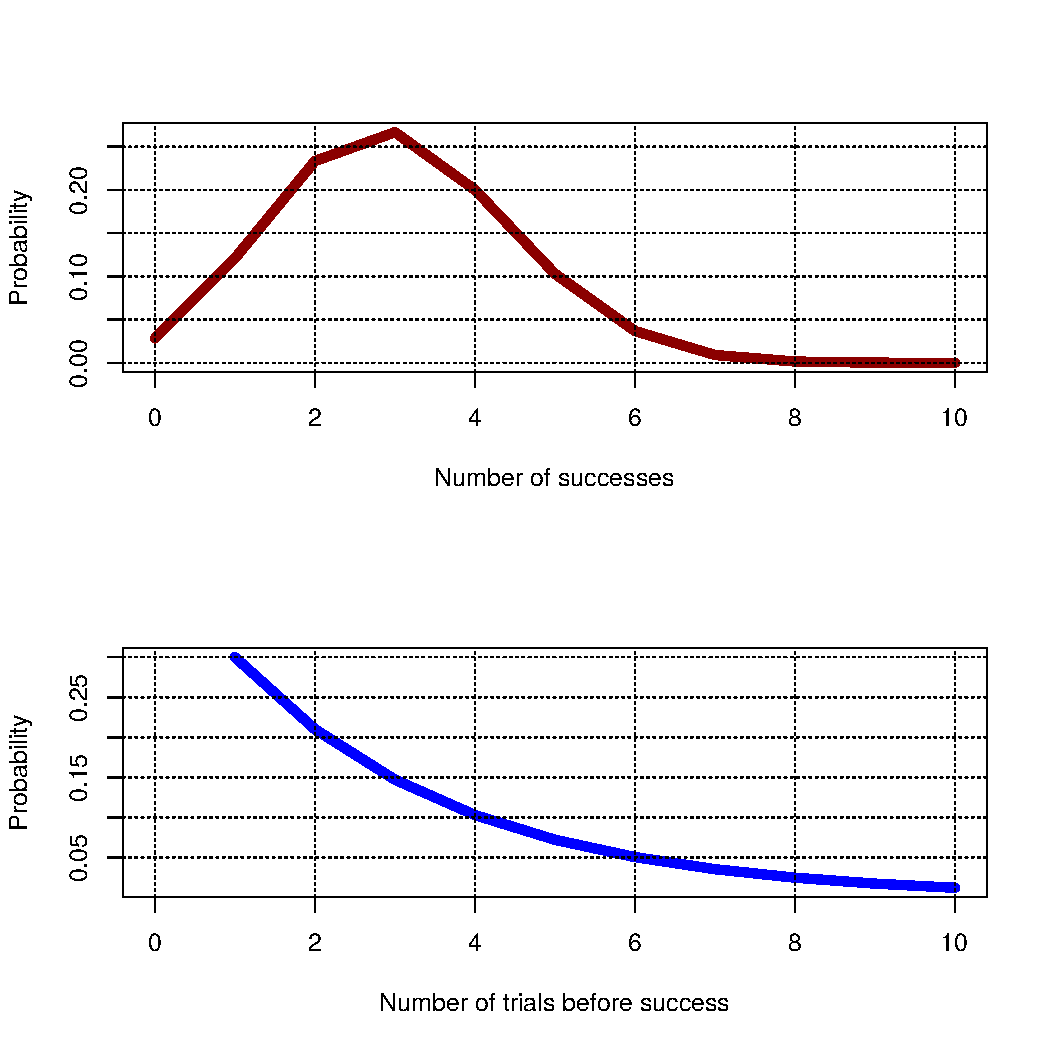
\includegraphics[width=0.6\textwidth]{graphics/distributions.pdf}
\caption{Геометрическое (нижний график) и биномиальное (верхний график) распределения вероятностей}
\label{fig:distributions}
\end{figure}

Таким образом, геометрическое распределение (здесь $p$ - это 
вероятность успеха в испытание, а $m \in \{1, 2, 3, 4, 5, \ldots\}$ - это 
количество попыток до первой удачи) можно обозначить следующей 
формулой:

$$P(X=m)=p(1-p)^{m-1}$$

Математические ожидания можно вычислять с помощью так называемых 
генерирующих функций. Так, для геометрического закона распределения 
вероятностей математическое ожидание можно найти следующим образом.
Для начала найдем математическое ожидание $E[e^{Xt}]$:

\eat{$$E[X]=\sum_{m=1}^\infty m p(1-p)^{m-1}=
p\sum_{m=1}^\infty \frac{dq^{m}}{dq}=
p\frac{d}{dq}\sum_{m=1}^\infty q^{m}=
p\frac{d}{dq} \frac{q}{1-q}=
\frac{1}{p}$$
}

$$m_X(t) = E[e^{Xt}] = \sum_{m=1}^{\infty} e^{mt}pq^{m-1} = 
\frac{p}{q}\sum_{m=1}^{\infty} (e^{t}q)^{m} = p\frac{e^t}{(1-e^tq)}$$

Далее вычислим производную функции $f(t)$:

$$\frac{d}{dt}m_X(t) = p\frac{e^t}{(1-e^tq)^2}$$

Вычислив производную в $t=0$ получим математическое ожидание для
геометрического закона распределения:

$$\frac{d}{dt}m_X(0) = E[X] = p\frac{1}{(1-q)^2}=\frac{1}{p}$$

Биномиальный же закон распределения вероятностей (здесь $p$ - это вероятность успеха, 
$m$ - это количество удач, а $n$ - это количество всех испытаний) можно выразить через 
следующую формулу:

$$P(X=m)=C^m_np^{m}(1-p)^{n-m}$$

Для данного закона распределения справедлива следующая формула математического 
ожидания $E[X]=\sum_{m=0}^n mC^m_np^{m}(1-p)^{n-m} = np$.  Найдём математическое 
ожидание с помощью генерирующей функции. Так, например, найдем математическое 
ожидание $E[e^{Xt}]$:

$$m_X(t) = E[e^{Xt}] = \sum_{m=0}^n e^{mt}C^m_np^{m}(1-p)^{n-m} = (pe^t+q)^n$$

Далее, найдём производную полученного выражения:

$$\frac{d}{dt}m_X(t) = n(pe^t+q)^{n-1}pe^t$$

Вычислив полученное выражение в точке $t=0$ получаем: 

$$\frac{d}{dt}m_X(0) = E[X] = n(pe^0+q)^{n-1}pe^0 = np$$

\subsection{Зачем нужна теория вероятности в изучении алгоритмов?}

Часто на практике необходимо дать среднюю сложность алгоритма,
а не например, максимальную, или сложность получающуюся в худшем случае. 
И тут как правило не обойтись без знаний теории вероятности и 
математической статистики. Приведем пример того как можно 
проанализировать сложность следующего алгоритма на языке Python:

\begin{python}
from random import randint

def collision(size = 100):
	x0 = randint(0, size);
	while True:
		x1 = randint(0, size);
		if x0 == x1:
			break;
\end{python}

Данный алгоритм ищет коллизии и прекращается тогда, когда найдено совпадение. Проанализируем
вычислительную сложность. Можем заметить, что вероятность нахождения совпадения на каждом шаге
равна $P(A) = p = \frac{1}{n}$, где $n$ - это общее количество ячеек или урн. Соответственно вероятность
того, что совпадения не будет, равна $P(\bar{A})=q=1-p$. Тогда вероятность 
коллизии на $i$-ом шаге можно вычислить как $P(X=i)=pq^{i-1}$.
Заметим, это распределение подчинено геометрическому закону.
Зная, что среднее значение геометрического распределения равно 
$E[X] = \sum_{i=1}^{\infty} ipq^{i-1} = \frac{1}{1-q}$, 
можно утверждать, что сложность данного алгоритма 
$\Theta(\frac{1}{1-q})$ (здесь мы говорим о среднем значение, а не о худшем случае или
лучшем случае, так как в худшем случае алгоритм может вообще не закончить свое 
выполнение, а в лучшем случае алгоритм может остановиться после первого шага).

Приведем еще один пример стохастического алгоритма. Пусть задача состоит в нахождении
случайной перестановки чисел из множества. Например, пусть дано множество $\{1, 2, 3\}$, 
тогда возможными перестановками будут  $\{1, 2, 3\}$, $\{2, 1, 3\}$, $\{1, 3, 2\}$,
$\{3, 2, 1\}$, $\{3, 1, 2\}$, $\{2, 3, 1\}$. Приведем (неэффективную) реализацию 
алгоритма (эффективный алгоритм требует время $O(n)$).

\begin{python}
from random import randint

def permutations(n):
	result = [0] * n;
	used = [False] * n;
	j = randint(0, n);
	used[j] = True;
	result[0] = j;
	for i in range(1, n):
		while True:
			r = randint(0, n - 1);
			if not used[r]:
				result[i] = r;
				used[r] = i;
				break;
	return result;
\end{python}

Заметим, что на $i$-ом шаге вероятность нахождения незанятого слота составляет 
$P(A) = p = \frac{n-i}{n}$ (вероятность обратного события будет 
$P(\bar{A}) = q = 1 - p =\frac{i}{n}$). Очевидно, что как и в предыдущем примере, 
вероятность того, что свободная ячейка найдется после $j$-ой итерации на $i$-ом 
шаге, будет равна $P(X=j)=pq^{j-1}$. Составим таблицу, в которой приведем 
ожидаемое время выполнения алгоритма на каждом шаге (смотрите Таблицу~\ref{tab:permutations}).

\begin{table}
\centering
\begin{tabular}{|c|c|c|c|}
\hline
Шаг & $P(A) = p$ & $P(\bar{A}) = q$ & Мат. ожидание  \\\hline
$1$ &  $(n-1)/n$      & $1/n$           & $\sum_{j=1}^{\infty} jpq^{j-1} = \frac{1}{(1-q)} = \frac{n}{(n-1)} $ \\\hline
$2$ &  $(n-2)/n$      & $2/n$           & $\sum_{j=1}^{\infty} jpq^{j-1} = \frac{1}{(1-q)} = \frac{n}{(n-2)} $ \\\hline
$3$ &  $(n-3)/n$      & $3/n$           & $\sum_{j=1}^{\infty} jpq^{j-1} = \frac{1}{(1-q)} = \frac{n}{(n-3)} $ \\\hline
$\ldots$ & $\ldots$   & $\ldots$        & $\ldots$ \\\hline
$i$ &  $(n-i)/n$      & $i/n$           & $\sum_{j=1}^{\infty} jpq^{j-1} = \frac{1}{(1-q)} = \frac{n}{(n-i)} $ \\\hline
\end{tabular}
\caption{Пошаговое вычисление ожидаемого времени выполнения алгоритма нахождения перестановок}
\label{tab:permutations}
\end{table}

\begin{figure}[ht!]
\centering
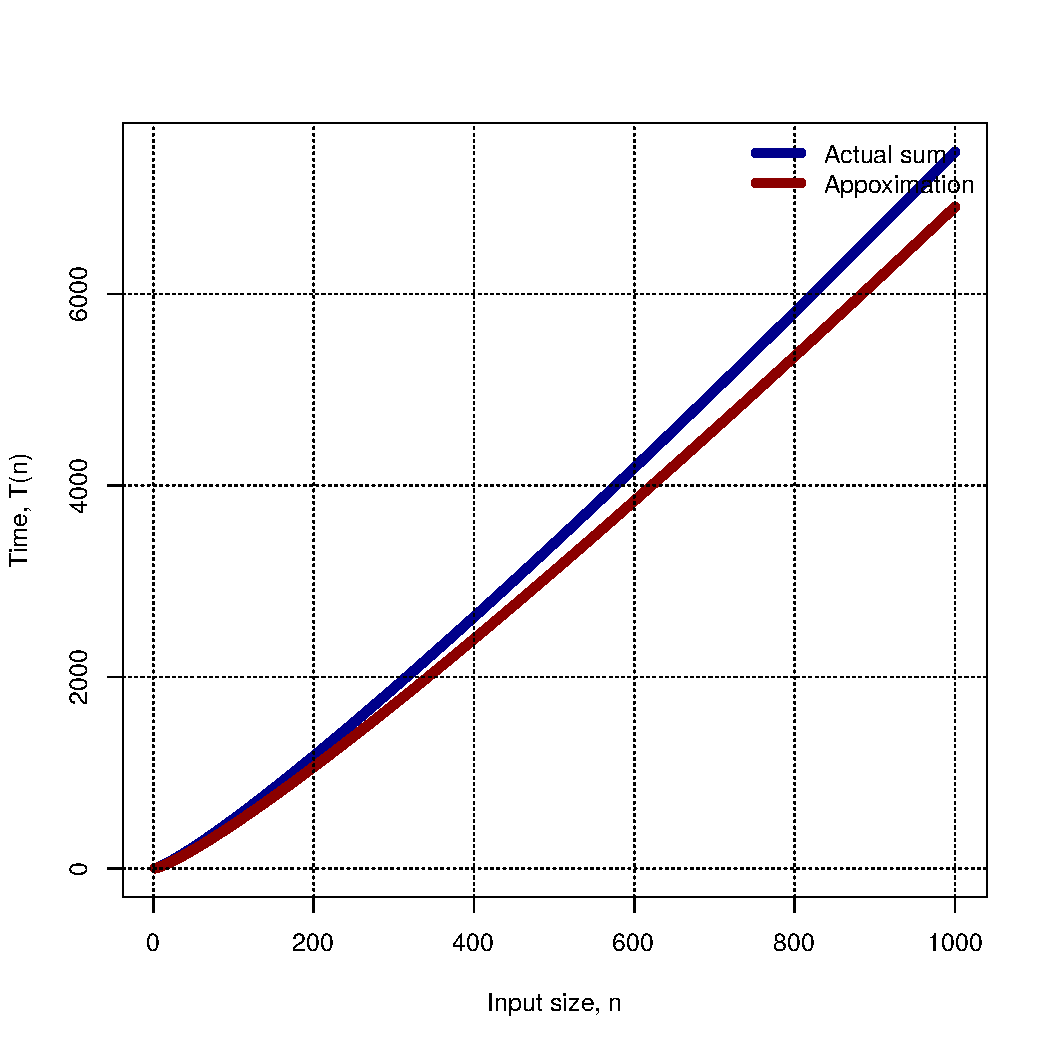
\includegraphics[width=0.6\textwidth]{graphics/approximation.pdf}
\caption{Сравнение точного значения суммы и аппроксимации}
\label{fig:approximation}
\end{figure}


Очевидно, что ожидаемое время выполнения алгоритма на $i$-ом шаге равно $\frac{n}{n-i}$.
Тогда, просуммировав все значения в последней колонке, мы сможем найти среднее время всего алгоритма, 
т.е., $\sum_{i=1}^{n-1}\frac{n}{(n-i)}$. Так как вычисление этой суммы достаточно сложно, то 
проще дать верхнюю оценку алгоритма, например $O(n^2)$. Здесь мы продемонстрировали не только как можно 
проводить анализ стохастического алгоритма, но и тот факт, что иногда проще дать верхнюю оценку
алгоритма, как мы упомянули это в Главе~\ref{sec:complexity}. Читатель может самостоятельно
попробовать дать точную оценку $\Theta$. Однако, заметив, что данная сумма напоминает 
гармонический ряд, мы можем аппроксимировать сумму интегралом 
(на Графике~\ref{fig:approximation} отображено расхождение реальной суммы и аппроксимации)
и тем самым дать нижнюю оценку сложности алгоритма:

$$\sum_{i=1}^{n-1}\frac{n}{(n-i)} \approx n\int_1^{n-1}\frac{dx}{(n-x)} = -nln(1)+nln(n-1) < n\log_2(n)$$

Тогда нижнюю границу для сложность нашего алгоритма можно оценить как $\Omega(n\ln(n))$.

\chapter{Основы языка программирования Python}

Прежде чем мы сможем окунуться в изучение алгоритмов и структур данных
нам необходимо ознакомиться с основами языка Python. Но начнем знакомство 
с Python с его установки.

\section{Установка Python3}

Установка интерпретатора Python достаточно простое действие, но оно отличается
в зависимости от того, какую операционную систему использует пользователь. 
Две наиболее распространённые операционные системы - это Windows от 
компании Microsoft, и бесплатно распространяемая операционная система 
Linux. Стоит отметить, что существует огромное множество дистрибутивов 
операционной системы Linux. Но в нашем случае, мы будем использовать 
дистрибутив Ubuntu.

\subsection{Установка в Windows}

Перед началом установки Python под управлением операционной системы
Windows, стоит выяснить разрядность процессора, который используется
для вычислений. Существует два основных типа процессора: $32$ битный 
(архитектура x86) и $64$ битный (архитектура x86-64).

После того как мы узнали разрядность процессора, заходим на официальный 
сайт Python \url{https://www.python.org/} и в разделе загрузок 
находим ссылку на последнюю версию языка Python. На момент написания 
данной книги последняя версия интерпретатора Python была $3.8.1$.

Скачиваем установщик интерпретатора для нужного типа процессора и после 
загрузки выполняем установку интерпретатора и среды разработки (для этого 
достаточно выполнить двойной щелчок по скаченному файлу). После установки
можно запустить командную строку (PowerShell) и выполнить слудующую команду:

\begin{verbatim}
C:\ > python
\end{verbatim}

Если установка прошла успешно, то пользователь должен увидеть приглашение 
интерпретатора для ввода команд.

\subsection{Установка в Linux}

Установка Python в Ubuntu Linux намного проще, так как можно воспользоваться
стандартным установщиком пакетов Ubuntu. Для этого стоит открыть консоль
и выполнить слудующую команду:

\begin{verbatim}
$ sudo apt-get install python3
\end{verbatim}

Менеджер пакетов самостоятельно загрузит интерпретатор Python, а также
все необходимые зависимости. После установки, можно проверить результат,
вызвав интерпретатор Python:

\begin{verbatim}
$ python3
\end{verbatim}

Стоит отметить, что вместе с интерпретатором установится и менеджер пакетов Python
- pip. Так, например, если нужно установить какую либо библиотеку, то это можно 
сделать с помощью программы pip. Например, если читатель хочет установить библиотеку
для работы с криптографическими примитивами (библиотека pycryptodome), то достаточно 
выполнить следующую команду:

\begin{verbatim}
$ pip3 install pycryptodome
\end{verbatim} 

В оставшейся части книги мы будем предполагать наличие именно Ubuntu Linux у 
пользователя. И все команды, которые мы будем приводить, будут исполняться в 
консоле (терминале) Ubuntu Linux.

Для демонстрации работы интерпретатора, предположим что пользователь создал
файл в редакторе (мы рекомендуем редактор SubLime~\footnote{https://www.sublimetext.com/}, 
так как он очень гибкий и подсвечивает синтаксис языка Python), ввел в него следующие строчки
кода (стоит заметить, что отступы должны быть либо табами, либо пробелами) и сохранил в 
домашней директории как hello\_world.py:

\begin{python}
from sys import argv

def main():
	print("Hello world, %s" % (argv[1]))

main()
\end{python}

После переходим в домашний каталог пользователя и выполняем наш первый скрипт:

\begin{verbatim}
$ cd ~
$ python3 hello_world.py Dmitriy
\end{verbatim}

После выполнения данных команд пользователь должен увидеть
\texttt{Hello world, Dmitriy} в консоле. Если такое сообщение не 
появится, то либо пользователь не правильно установил Python,
либо не корректно ввел исполняемый код, приведённый выше,
либо сохранил код не в нужной директории.

\section{Типы данных}

Язык Pyhton не строго типизированный, то есть для объявления
переменных не требуется указывать тип данных переменной. Но не смотря на
это в языке Python все же существует несколько типов данных.
Перечислим эти типы данных. Так в языке Python есть целочисленные данные,
численные данные с плавающей точкой, комплексные числа, булевы данные, строковые данные, а 
также объекты. Существуют встроенные и пользовательские объекты. Так например, к
встроенным объектам можно отнести последовательности (списки, кортежи), 
словари, множества, а также бинарные объекты (байты и байтовые массивы).

Приведем примеры этих типов данных. Начнём с целочисленных данных. 
Целочисленные данные представляют собой множество натуральных чисел. Как и в 
математике, в Python3 целочисленная переменная может принимать любое значение 
от минус бесконечности до плюс бесконечности (конечно объём доступной памяти
накладывает ограничения). Это нововведение в Python3 позволяет 
работать с большими числами без особого труда. В частности, это свойство незаменимо 
в криптографических алгоритмах. Приведём пример объявления цулочисленной переменной. 
Для этого дадим сначала имя переменной и присвоим ей значение $10$, как это указано 
в нашем примере:

\begin{python}
number = 10
\end{python}

Теперь переменная \texttt{number} содержит данные в виде числа $10$. Целые числа
можно задавать и в системе счисления отличной от десятичной. Например, число $10$ можно задать
в двоичной системе счисления:

\begin{python}
number = 0b1010
\end{python}

Или же можно задать это же число в шестнадцатеричной системе счисления:

\begin{python}
number = 0xA
\end{python}

Стоит заметить, что переменной \texttt{number} можно присвоить значение
любого другого типа данных. Например, следующие выражения являются корректными
в языке Python:

\begin{python}
number = 10;
number = 10.1;
\end{python}

Следующий тип данных, который мы рассмотрим будут числа с плавающей точкой.
Такие числа можно представить как в явном виде, так и в научном. Например,
следующая строчка кода инициализирует переменную числом с плавающей точкой 
в явном виде:

\begin{python}
number = 2.718;
\end{python}

Можно также использовать научный формат для данных с плавающей точкой.
Например, число $3\cdot10^{10}$ можно записать в языке Python как:

\begin{python}
number = 3e10;
\end{python}

Если же потребуется задать число с определённым числом знаков после запятой, т.е., представить, например, 
число вида $278\cdot10^{-2}$, то можно воспользоваться следующей нотацией:

\begin{python}
number = 278e-2;
\end{python} 

Для данных с плавающей точкой существуют ограничения. Таким образом, максимальное
значение для данных с плавающей точкой будет число $1.7976931348623157\cdot10^{308}$

\begin{python}
number = 1.7976931348623157e308;
\end{python}

Число, которое больше $1.7976931348623157\cdot10^{308}$ уже будет равно 
бесконечности (для этого существует специальная 
константа \texttt{inf}). Тоже самое ограничение существует и для отрицательных чисел,
т.е., минимальное значение будет $-1.7976931348623157\cdot10^{308}$, а все что меньше этого числа будет равно 
минус бесконечности (или же \texttt{-inf}). Более того, если число меньше $10^{-323}$,
то оно будет равно $0.0$. Например, если читатель выполнит следующую команду в интерпретаторе,
то он получит число ноль:

\begin{python}
number = 1e-324
\end{python}

Вообще, строго говоря, приведённые примеры выше имеют смысл для компьютеров с 64 
битной архитектурой (автор книги использует именно такой процессор). Читатель
может самостоятельно проверить максимальное и минимальное значения для данных с плавающей 
точкой, выполнив следующий код:

\begin{python}
import sys
sys.float_info
\end{python}

Строковые данные в Python3 представляют собой набор символов, 
закодированных в UTF-8~\cite{} формате. Строковые переменные должны всегда 
быть заключены в одинарные или двойные кавычки. Например, 
объявить строковые переменные можно следующим образом:

\begin{python}
my_string_var = 'Python is great!';
my_string_var = "Python is great!";
\end{python}

В языке Python существует набор специальных функций для работы со строками.
Рассмотрим наиболее часто используемые из них. Для того, чтобы получить 
справку по всем доступным функциям для работы со строками достаточно выполнить 
следующую команду в интерпретаторе:

\begin{python}
help(str)
\end{python}

\section{Переменные}

\section{Операторы}

\subsection{Бинарные операторы}

Бинарные операторы это те операторы, которые требуют два операнда - левый и 
правый. Например, сложение двух целых числ требует бинарный оператор $+$:

\begin{python}
def add(operand1, operand2):
	return operand1 + operand2;
result = add(10, 12);
\end{python}

\subsubsection{Сложение}

\subsubsection{Вычитание}

\subsubsection{Умножение}

\subsubsection{Деление}

\subsubsection{Остаток от деления}

Каждое число $a$ можно представить в виде следующей линейной комбинации: $a=bq+r$.
Тогда если мы будем делить $a$ на $b$, то $r$ будет остатком от деления. В языке Python
остаток от деления можно получить используя оператор $\%$.

Часто бывает необходимо вычислить остаток от деления двух целых чисел. Например,
в теории чисел, которая используется в криптографии бывает необходимо вычислить 
наибольший общий делитель двух чисел, $gcd(a, b)$. Для этого используют широко известный 
алгоритм Евклида, который был бы немыслимый без оператора, который даёт
остаток от деления. Приведем этот алгоритм:

\begin{python}
def gcd(a, b):
	if b == 0:
		return a;
	return gcd(b, a % b);
\end{python}

\subsection{Унарные операторы}

\subsection{Логические операторы}

\subsection{Приоритеты операторов}

\section{Выражения}

\section{Циклы}

\begin{python}
i = 10;
while i >= 0:
  print("Current index: " + str(i));
  i -= 1;
\end{python}

\begin{python}
end = 10;
start = 0;
step = 1;
for i in range(start, end, step):
  print("Current index: " + 0);
\end{python}

\section{Ветвления}

\begin{python}
from sys import stdin
a = 10;
print("Input a number: ")
b = int(stdin.readline())
if a > b:
	print("a > b")
elif a == b:
	print("a == b")
else:
	print("a < b")
\end{python}

\section{Функции}

\section{Классы}

\section{Модули}

\chapter{Основные структуры данных}

\section{Множества}

\section{Массивы}

\section{Ассоциативные массивы}

\section{Очереди, стеки, кучи}

Рассмотрим бинарную кучу, которую мы приводим на Графике~\ref{fig:binary_heap}. Прежде чем 
мы приступим описаню свойств бинарной кучи и тому, как бинарная куча может быть реализована в 
языке Python, приведем теорему, результат который позволяет эффективно обходить бинарное дерево. 

\begin{figure}
\centering
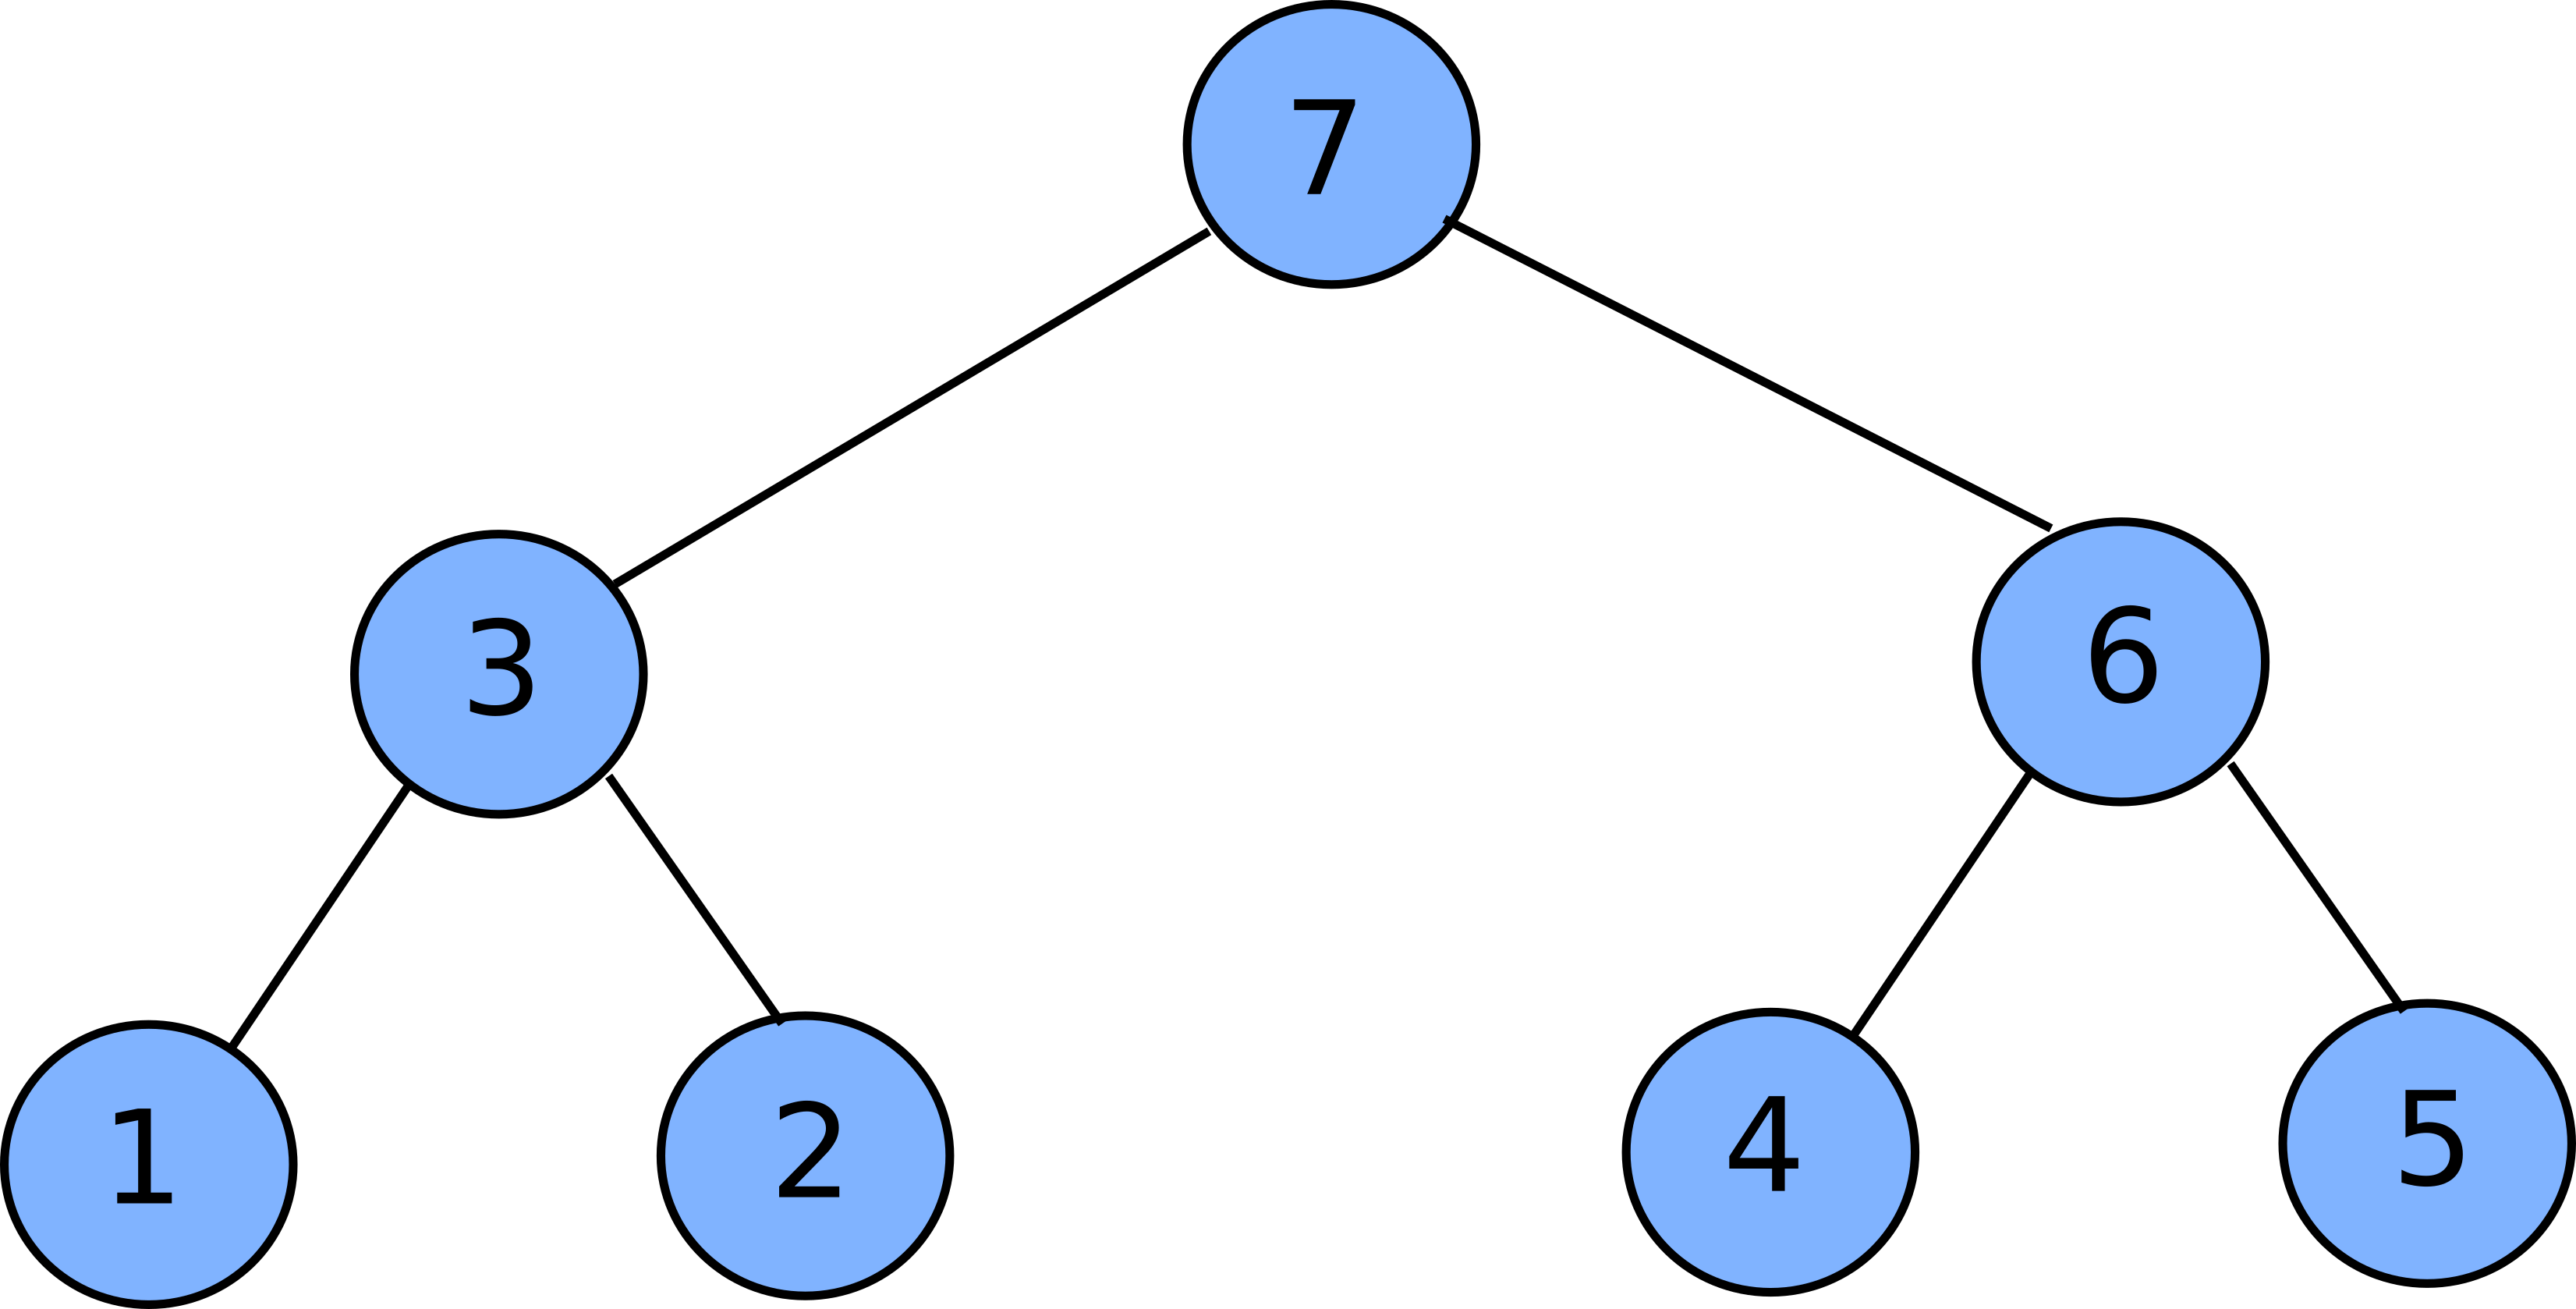
\includegraphics[width=0.6\textwidth]{graphics/binary_heap.png}
\caption{Бинарная куча}
\label{fig:binary_heap}
\end{figure}

\begin{theorem}
В сбалансированном бинарном дереве левый потомок $i$-ого узла может быть найден под 
индексом $2i$, а правый потомок под индексом $2i+1$.
\end{theorem}

Пусть нам дан узел дерева с индексом $i$ (индексирование узлов начинается с $1$). Тогда глубина этого узла 
будет равна $\lfloor \log_2(i) \rfloor$ (это очевидно, так как на каждом 
уровне количество узлов удваивается, см. График~\ref{fig:binary_heap}). Пусть $n$ - это количество узлов, 
предшествующих узлу $i$ (на том же уровне), а $m$ - это общее количество узлов
до текущего уровня $\lfloor \log_2(i) \rfloor$ включительно. Тогда индекс 
левого потомка можно вычислить как $2n + m+1$. Но так как
$$n = i - \sum_{l=0}^{\lfloor \log_2(i) \rfloor - 1} 2^l - 1 = i - (2^{\lfloor \log_2(i) \rfloor} - 1) - 1$$ 
A так как
$$m=\sum_{l=0}^{\lfloor \log_2(i) \rfloor} 2^l = 2^{\lfloor \log_2(i) \rfloor + 1} - 1$$
Получаем
$$2n+m+1= 2(i - (2^{\lfloor \log_2(i) \rfloor} - 1) - 1) + 2^{\lfloor \log_2(i) \rfloor + 1} - 1 + 1 = 2i$$ 

Очевидно, что индекс правого потомка тогда будет равен $2i+1$.
Что и требовалось доказать.

Отметим способ, которым мы нашли сумму. Пусть $S=\sum_{l=0}^{\lfloor \log_2(i) \rfloor} 2^l$, тогда 
$2S=\sum_{l=1}^{\lfloor \log_2(i) \rfloor + 1} 2^l$, а $2S-S = 2^{\lfloor \log_2(i) \rfloor + 1} - 1$.


Рассмотрим добавление узла в бинарную кучу~\ref{fig:binary_heap_insertion}.

\begin{figure}
%\centering
\begin{subfigure}[t]{0.6\textwidth}
	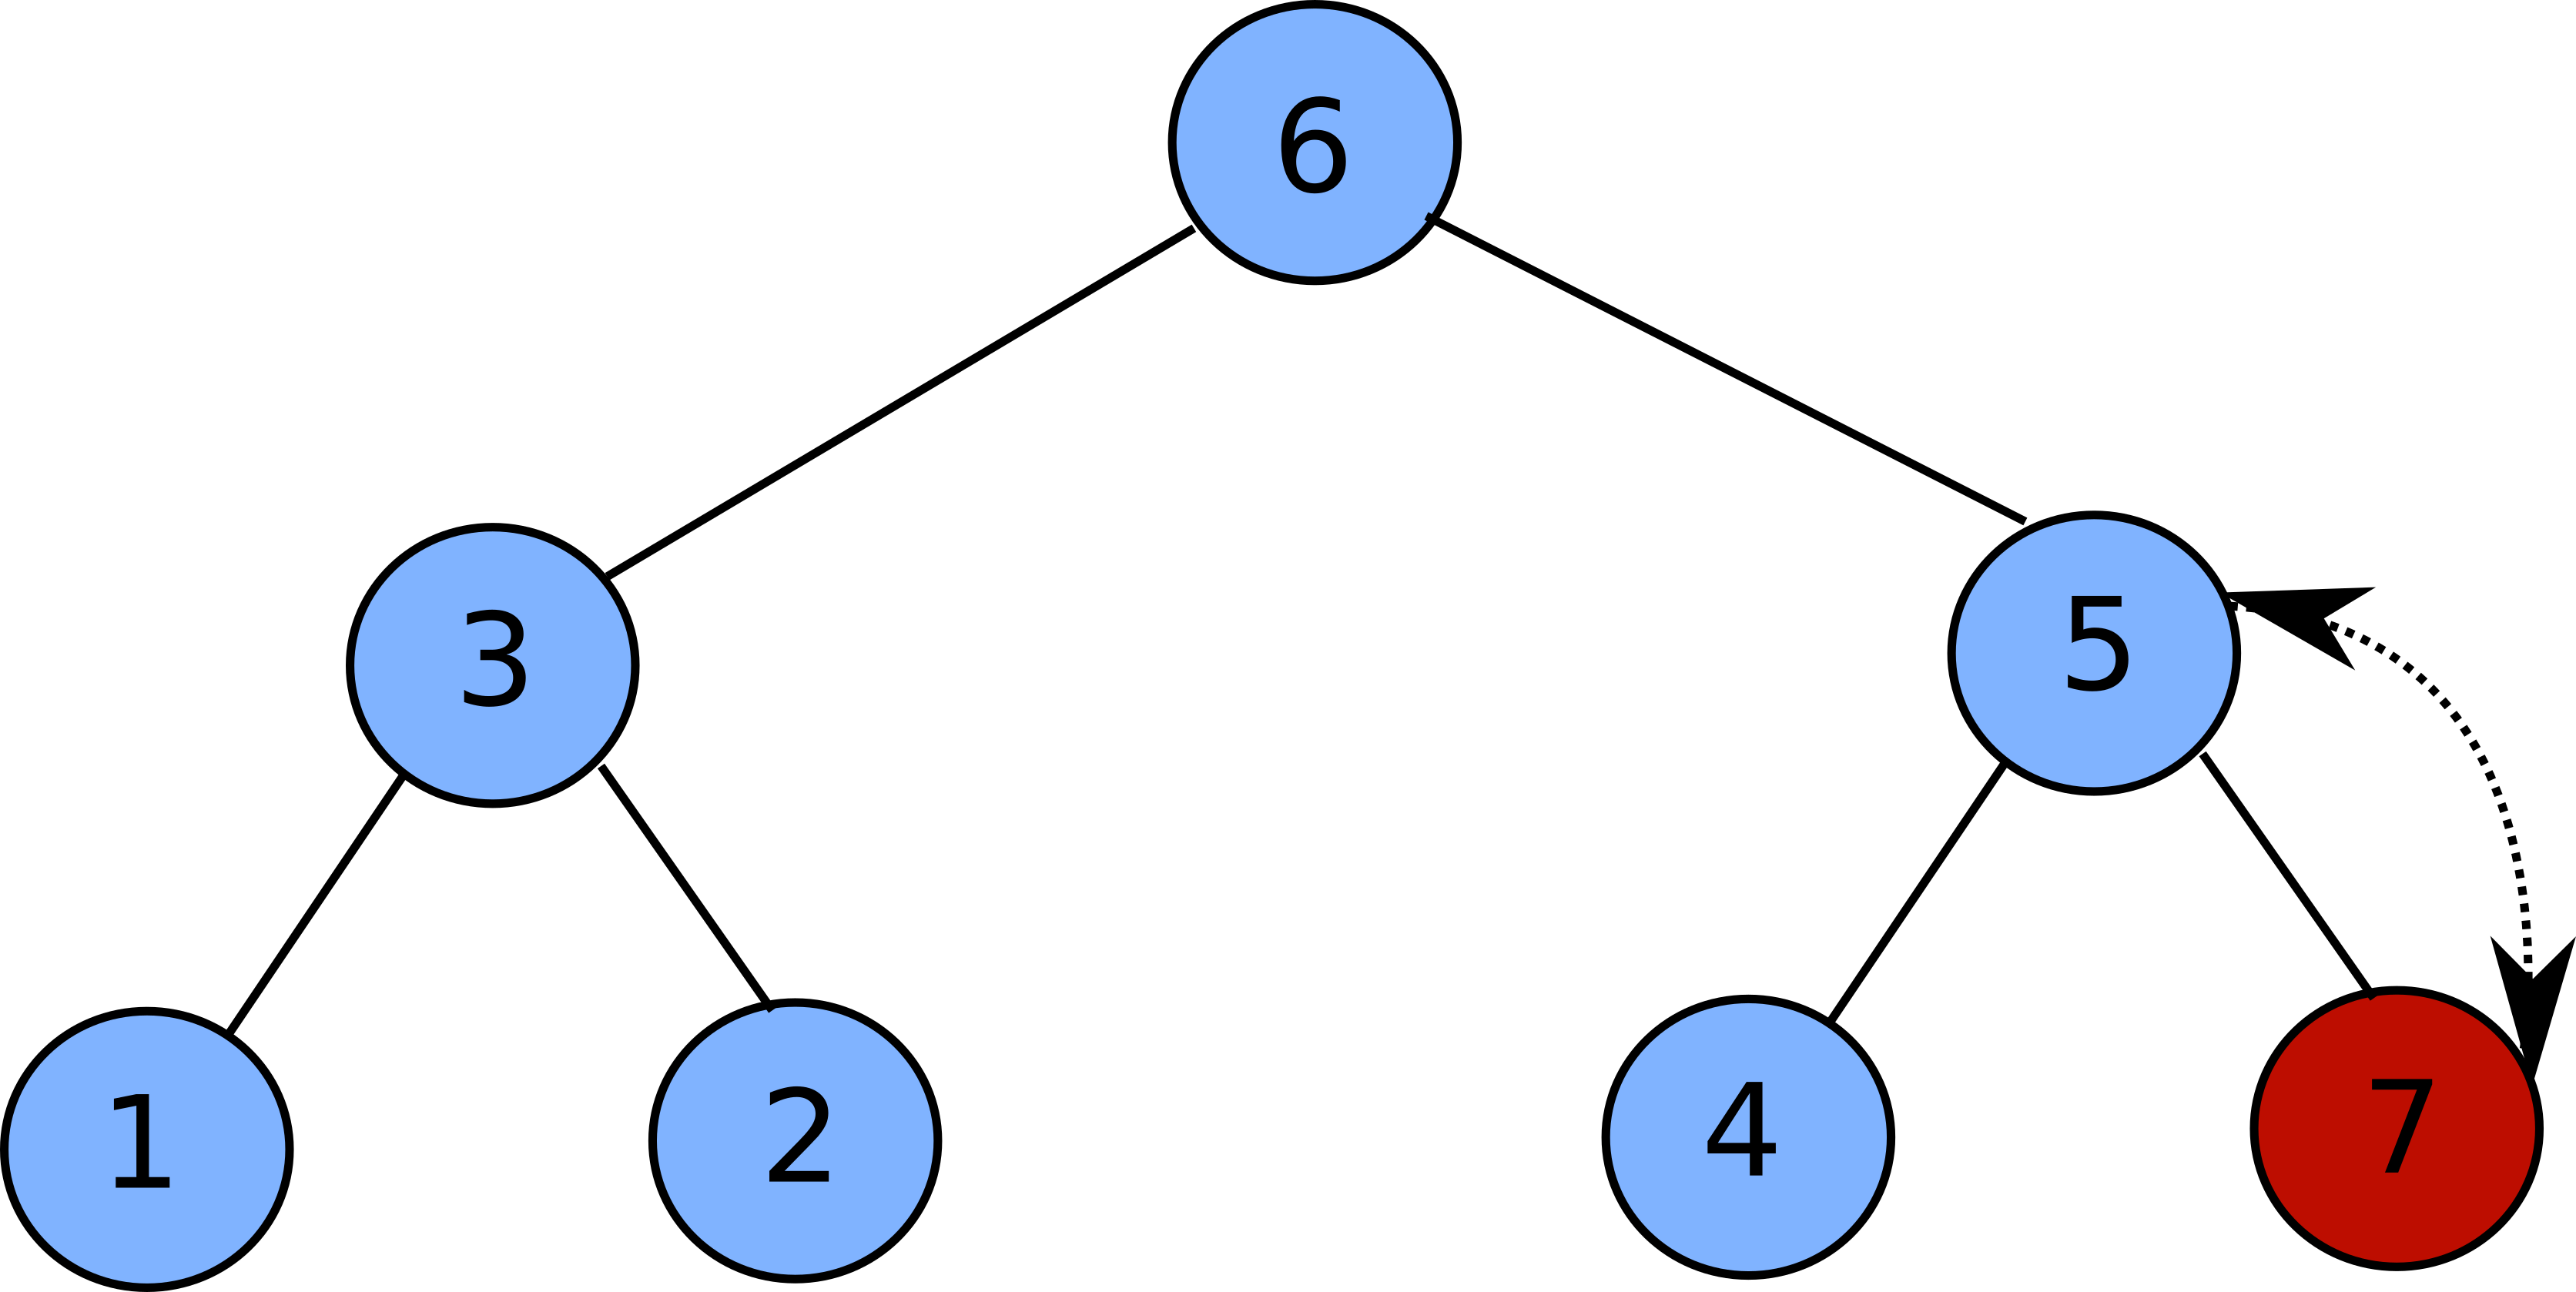
\includegraphics[width=0.8\textwidth]{graphics/binary_heap_insert_1.png}
\end{subfigure}
\begin{subfigure}[t]{0.6\textwidth}
	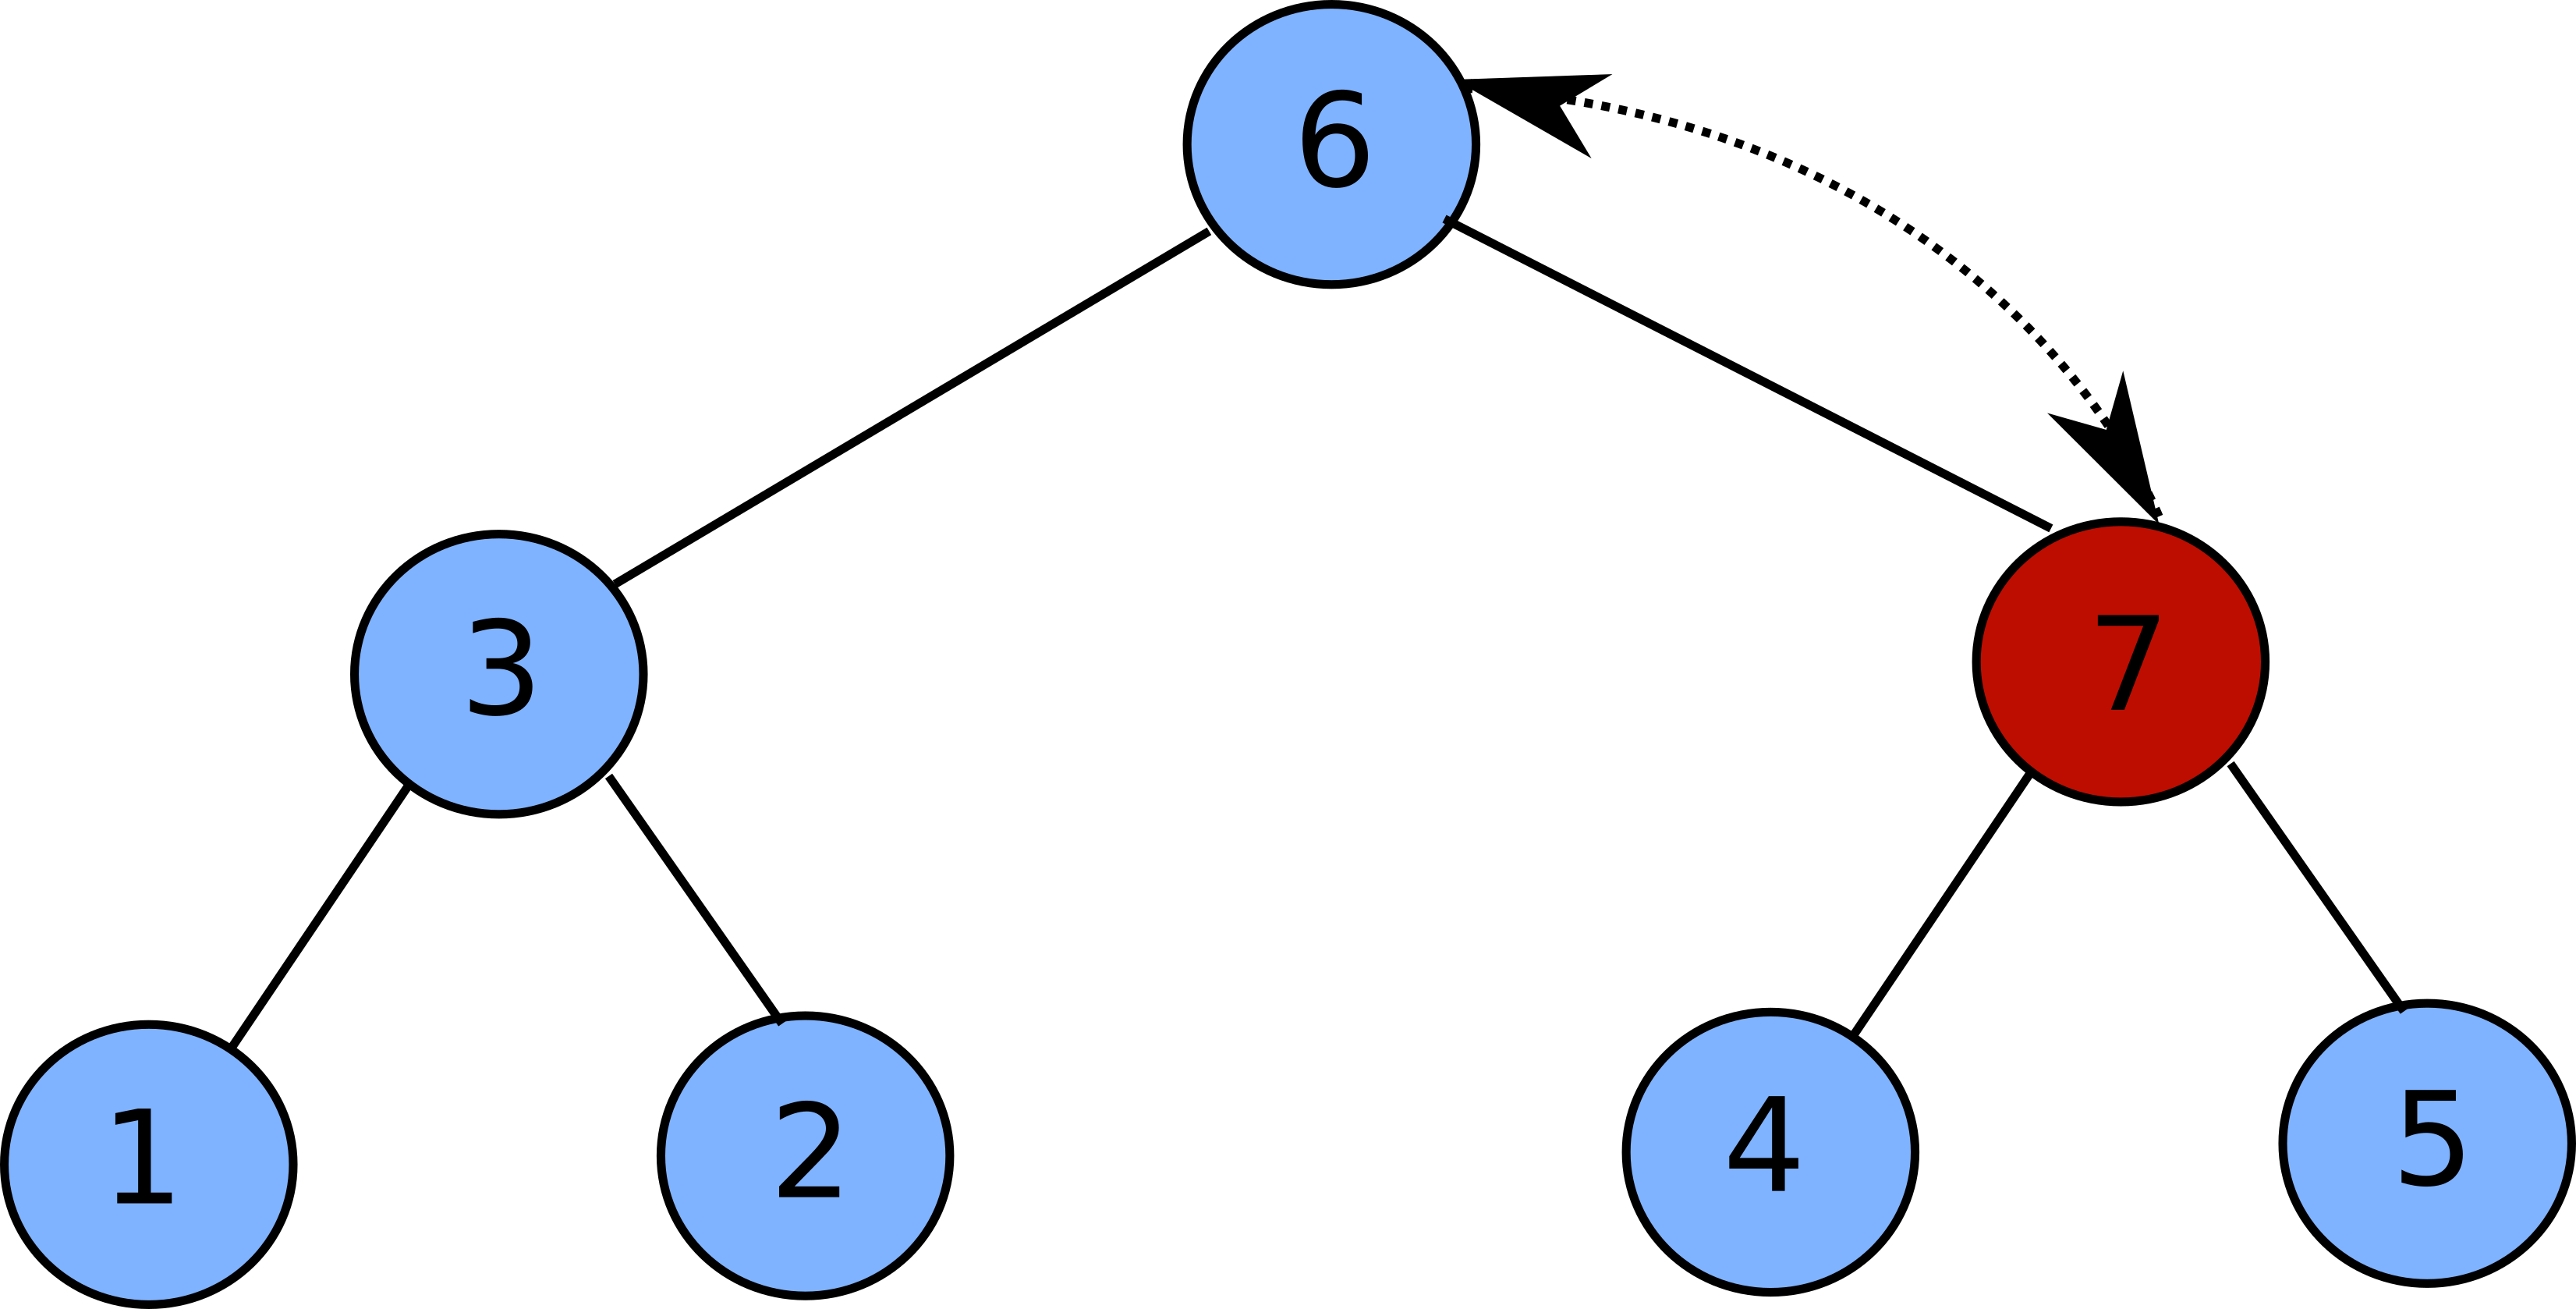
\includegraphics[width=0.8\textwidth]{graphics/binary_heap_insert_2.png}
\end{subfigure}
\caption{Добавление элемента к бинарной куче}
\label{fig:binary_heap_insertion}
\end{figure}

\begin{python}
class heap():
	def __init__(self):
		self.h = [0];
		self.length = 0;

	def size(self):
		return self.length;

	def _down(self):
		c = 1;
		while c * 2 <= self.length:
			if c * 2 + 1 <= self.length:
				if self.h[c * 2] < self.h[c * 2 + 1] 
					and self.h[c] < self.h[c * 2 + 1]:
					v = self.h[c];
					self.h[c] = self.h[c * 2 + 1];
					self.h[c * 2 + 1] = v;
					c = c * 2 + 1;
				elif self.h[c] < self.h[c * 2]:
					v = self.h[c];
					self.h[c] = self.h[c * 2];
					self.h[c * 2] = v;
					c = c * 2;
				else:
					break;
			else:
				if self.h[c] < self.h[c * 2]:
					v = self.h[c];
					self.h[c] = self.h[c * 2];
					self.h[c * 2] = v;
					c = c * 2;
				else:
					break;

	def _up(self):
		c = self.length;
		while c > 1 and self.h[c] > self.h[floor(c / 2)]:
			v = self.h[c];
			self.h[c] = self.h[floor(c / 2)];
			self.h[floor(c / 2)] = v;
			c = floor(c / 2);

	def pop(self):
		if self.length == 0:
			return None;
		self.length -= 1;
		v = self.h[1];
		if self.length == 0:
			self.h = [0];
			return v;
		self.h[1] = self.h[len(self.h) - 1];
		self.h = self.h[0:len(self.h) - 1];
		self._down();
		return v;

	def push(self, v):
		self.length += 1;
		self.h.append(v);
		self._up();
\end{python}

\section{Деревья}

\subsection{Бинарные деревья}

\subsection{Сбалансированные бинарные деревья}

\subsection{Обход дерева вглубь и вширь}

\section{Графы}

\subsection{Направленные графы}

\subsection{Ненаправленные графы}

\subsection{Представление графов в Python}

\subsection{Обход графов}

\subsection{Поиск наикратчайшего пути между двумя вершинами}

\chapter{Базовые алгоритмы}

В данном разделе мы рассмотрим основные алгоритмические приёмы 
для решения вычислительных задач. 

\section{Разделяй и властвуй}

Основной подход алгоритмов данной категории заключается 
в деление входных данных на части до тех пор пока задача 
не сведётся к тривиальной. После обработки данных, в 
зависимости от алгоритма, данные могут быть объединены 
воедино для решения поставленной задачи. Например, 
в алгоритмах сортировки, данные делятся на 
сегменты до тех пор пока их размеры не будут 
настолько малы, что потребуют $O(1)$ времени 
на их обработку. В эту же категорию попадают 
алгоритмы, которые делят входные данные пополам
до тех пор пока не будет найдено решение. Примером
таких алгоритмов могут быть бинарный поиск и 
метод бисекций, которые мы рассмотрим далее.

\subsection{Бинарный поиск}

\begin{python}
def binary_search(a, v):
	a = quicksort(a);
	target = v;
	start = 0;
	end = len(a) - 1;
	if len(a) == 0:
		return None;
	while True:
		if end - start == 1 or end == start:
			if a[start] == v:
				return (start, v);
			elif a[end] == v:
				return (end, v);
			else:
				return None;
		mid_point = floor((end + start) / 2);
		if target < a[mid_point]:
			end = mid_point;
		elif target > a[mid_point]:
			start = mid_point;
		elif target == a[mid_point]:
			return (mid_point, v);
\end{python}



\subsection{Метод бисекции}

Метод бисекции - это численный метод приближенного решения уравнений.
Данный метод является хорошим примером того, как работает метод разделяй и властвуй:
на каждом шаге размер входных данных уменьшается вдвое и алгоритм продолжает 
свое выполнение пока не будет найдено решение (точнее не будет достигнут 
порог). \eat{Конечно, как мы увидим позже в следующих параграфах мы будем иметь дело 
немного с другими алгоритмами. Например, в методе сортировки слиянием,
несмотря на то, что входные данные на каждом шаге делятся на две части,
алгоритм не отбрасывает часть данных, а лишь работает с каждой по отдельности.}

\begin{python}
def f(x):
	return x*x - 2*x;
def bisection(f, a, b, epsilon):
	while True:
		y0 = f(a);
		y1 = f(b);
		y2 = f((a+b)/2);
		if (y1 > 0 and y2 < 0) or (y1 < 0 and y2 > 0):
			a = (a+b)/2;
		elif (y0 > 0 and y2 < 0) or (y0 < 0 and y2 > 0):
			b = (a + b)/2;
		else:
			raise Exception("Signs are the same on both ends");
		if abs(a-b) <= epsilon:
			return (a + b)/2;

print(bisection(f, 0.1, 3, 0.000001));
\end{python}

% 4 2 1 1/2 1/4 1/8 1/6 /32
% log(8-0)+abs(log(1/32))
Дадим более строгое определение методу половинного 
деления, или методу бисекции. Пусть функция $f(x)$ непрерывна
на интервале $[a, b]$ и $f(a)f(b)<0$, т.е. знаки функции
в точках $a$ и $b$ разные. Разделим отрезок $[a, b]$ пополам,
и пусть $\gamma$ есть середина этого отрезка. Тогда, если
$f(\gamma) = 0$ (или близко к нулю), то $\gamma$ и есть
искомый корень (в нашем же случае мы останавливаем вычисления,
если длина нового отрезка меньше заданного порога $\epsilon$, что в принципе
эквивалентно). Иначе, через $[a_1, b_1]$ обозначим ту из половин
$[a, \gamma]$ или $[\gamma, b]$, на концах которой функция имеет
противоположенные знаки, и алгоритм продолжается.


Проанализируем вычислительную сложность данного алгоритма. 
Пусть $|a-b|>1$, тогда сложность алгоритма можно представить в виде 
следующей суммы: $\log_2(|a-b|) + |\log_2(\epsilon)|$. Но так как 
мы предполагаем, что $\log_2(|a-b|)$ является достаточно 
малой величиной, то сложность алгоритма можно выразить как 
$O(|log_2(\epsilon)|)$.


\subsection{Сортировка слиянием}

\begin{python}

from math import floor

def merge(a, b):
	c = [];
	h = 0;
	l = 0;
	while h < len(a) and l < len(b):
		if a[h] < b[l]:
			c.append(a[h]);
			h += 1;
		else:
			c.append(b[l]);
			l += 1;
	if h < len(a):
		for j in range(h, len(a)):
			c.append(a[j]);
	if l < len(b):
		for j in range(l, len(b)):
			c.append(b[j]);
	return c;

def merge_sort(a):
	if len(a) <= 1:
		return a;
	midpoint = floor(len(a) / 2);
	w = merge_sort(a[0:midpoint]);
	v = merge_sort(a[midpoint:len(a)]);
	return merge(w, v);
\end{python}

\subsection{Быстрая сортировка}

\begin{python}
def quicksort(a):
	if len(a) == 1:
		return a;
	if len(a) == 0:
		return [];
	midpoint = floor(len(a) / 2);
	smaller = [];
	larger  = [];
	for i in range(0, len(a)):
		if i == midpoint:
			continue;
		if a[midpoint] > a[i]:
			smaller.append(a[i]);
		if a[midpoint] <= a[i]:
			larger.append(a[i]);
	left = quicksort(smaller);
	right = quicksort(larger);
	return left + [a[midpoint]] + right;
\end{python}

\subsection{Сортировка кучей}

\begin{python}
def heap_sort(a):
	h = heap();
	for i in a:
		h.push(i);
 +	b = [];
	for i in range(0, h.size()):
		b.append(h.pop());
	b.reverse();
	return b;
\end{python}

\section{Жадные алгоритмы}

\subsection{Коды Хафмана}

\section{Динамическое программирование}

Динамическое программирование является мощным инструментом 
при разработке программ. Основная мысль данного подхода заключается 
в разбиение одной сложной задачи на более простые подзадачи и запоминание 
результатов вычислений этих подзадач в одномерном или двумерном массиве. 
После решения подзадач, можно перейти к решению более общей задачи и найти тем 
самым оптимальное решение для общей задачи. Самое главное преимущество динамического
программирования заключается в том, что этот метод позволяет существенно снизить 
вычислительную сложность: так как для решения более общей подзадачи используются
сохранённые решения подзадач, то вычислительная сложность заметно сокращается. 

Рассмотрим применение динамического программирования на примере вычислений чисел Фибоначчи. Числа 
Фибоначчи могут быть вычислены рекурсивно следующим образом: $F_i = F_{i-1} + F_{i-2}$, 
где $F_0=0, F_1=1$. Например, на языке Python решение можно записать следующим образом:

\begin{python}
def fib(n):
	if n == 0:
		return 0;
	if n == 1:
		return 1;
	return fib(n - 1) + fib(n - 2);
\end{python}

Но рекурсия не эффективна в данном случае. Более того приведённый выше кусок кода 
является примером того, как не надо использовать рекурсию. Давайте проанализируем это 
рекурсивное решение. Очивидно, что:

$$
T(n) = T(n-1) + T(n-2) + 1
$$

Предполагая худший случай $T(n-2)=T(n-1)$, мы легко можем получить следующее решение:

\begin{equation*}
\begin{multlined}
T(n) = 2T(n-1) + 1= \\
	   2(2T(n-2) + 1) + 1 = 
	   \ldots = \\
	   2^{i}T(n-i) + 2^{i} - 1 = 
	   \ldots = \\
	   2^{n-1} + 2^{n-1} - 1 = 
	   2^{n} - 1
\end{multlined}
\end{equation*}

Как видно, вычислительная сложность данного рекурсивного алгоритма 
может быть представлена показательной функцией, т.е. $O(2^n)$. Рекурсия может 
быть заменена динамическим программированием. 
Так например, если мы будем запоминать в массиве значения $F_i$, то мы сможем
эффективно вычислить все последующие значения ($F_{i+1}$, $F_{i+2}$ и т.д), и 
вычислительная сложность будет линейной, т.е. $O(n)$. В языке Python задачу 
можно решить следующим образом:

\begin{python}
def fib(n):
	if n == 0:
		return 0;
	if n == 1:
		return 1;
	F = [0, 1];
	for i in range(2, n + 1):
		F.append(F[i - 1] + F[i - 2]);
	return(F[n]);
\end{python}


Рассмотрим более сложную задачу - нахождение наиболшей общей подстроки в двух строках.

$$
T[i][j] = \Bigg\{
	\begin{array}{cc}
      T[i - 1][j - 1] + 1 & if X[i] = Y[j] \\
      0 & otherwise \\
    \end{array}
$$

\begin{table}
\centering
\begin{tabular}{|c|c|c|c|c|c|}
	\hline
	&   & \cellcolor{blue}A & \cellcolor{blue}B & \cellcolor{blue}C & \cellcolor{blue}A \\\hline
	& \cellcolor{lightblue}0 & \cellcolor{lightblue}0 & \cellcolor{lightblue}0 & \cellcolor{lightblue}0 & \cellcolor{lightblue}0 \\\hline
	\cellcolor{blue}A & \cellcolor{lightblue}0 & \cellcolor{red}1 & \cellcolor{lightblue}0 & \cellcolor{lightblue}0 & \cellcolor{red}1 \\\hline
	\cellcolor{blue}B & \cellcolor{lightblue}0 & \cellcolor{lightblue}0 & \cellcolor{red}2 & \cellcolor{lightblue}0 & \cellcolor{lightblue}0 \\\hline
	\cellcolor{blue}A & \cellcolor{lightblue}0 & \cellcolor{red}1 & \cellcolor{lightblue}0 & \cellcolor{lightblue}0 & \cellcolor{red}1 \\\hline
\end{tabular}
\caption{Ход выполнения алгоритма нахождения наибольшей общей подстроки}
\end{table}

\begin{python}
def LCS(a, b):
	table = [0] * (len(a) + 1);
	for i in range(0, len(a) + 1):
		table[i] = [0] * (len(b) + 1);
	max_length = 0;
	end = 0;
	for i in range(1, len(a) + 1):
		for j in range(1, len(b) + 1):
			if a[i - 1] == b[j - 1]:
				table[i][j] = table[i - 1][j - 1] + 1;
				if table[i][j] > max_length:
					max_length = table[i][j];
					end = i;
	return a[end - max_length:end];
\end{python}

Очевидно что сложность данного алгоритма - $O(nm)$, где $m$ и $n$ - длины строк. 
Самая главная сложность в динамическом программирование - это увидеть оптимальную подзадачу
и грамотно составить рекуррентное выражение. 

Приведём еще один пример и остановимся более детально на том,
как составлять рекуррентное выражение. Для начала приведем описание 
проблемы. Пусть нам даны две строки, и мы хотим найти наименьшее 
число операций (таких как удаление, добавление или замена) необходимое для
превращения одной строки во вторую. 

%# +---+---+---+---+---+
%# |   |   | A | B | A |
%# +---+---+---+---+---+
%# |   | 0 | 1 | 2 | 3 |
%# +---+---+---+---+---+
%# | A | 1 | 0 | 1 | 2 |
%# +---+---+---+---+---+
%# | C | 2 | 1 | 1 | 2 |
%# +---+---+---+---+---+
%# | C | 3 | 2 | 2 | 2 |
%# +---+---+---+---+---+
%# | A | 4 | 3 | 3 | 2 |
%# +---+---+---+---+---+

%Пока не уверен, что правильно

$$
T[i][j] = min \Bigg\{
	\begin{array}{c}
      T[i - 1][j - 1] + diff(T[i], T[j])\\
      T[i - 1][j] + 1 \\
      T[i][j - 1] + 1 \\
    \end{array}
$$

\chapter{Финальный проект}

В данном разделе мы приведём финальный проект, который реализует построчное сравнение 
файлов. В данном проекте мы будем использовать принципы динамического программирования,
библиотеки для создания графического интерфейса - tkinter, а также 


\begin{python}
def reverse_string(a):
	r = ""
	for i in range(len(a) - 1, -1, -1):
		r += a[i];
	return r;

def diff(a, b):
	table = LCS(a, b);
	m = len(a); # (rows) 
	n = len(b); # (columns)
	r = "";
	while True:
		if n > 0 and m > 0 and a[m - 1] == b[n - 1]:
			r += a[m - 1];
			m = m - 1;
			n = n - 1;
		elif n > 0 and (m == 0 or table[m][n - 1] > table[m - 1][n]):
			r += "+" + b[n - 1];
			n = n - 1;
		elif m > 0 and (n == 0 or table[m][n - 1] <= table[m - 1][n]):
			r += "-" + a[m - 1];
			m = m - 1;
		else:
			break;
	return reverse_string(r);

def LCS(a, b):
	table = [0] * (len(a) + 1);
	for i in range(0, len(a) + 1):
		table[i] = [0] * (len(b) + 1);
	max_length = 0;
	end = 0;
	for i in range(1, len(a) + 1):
		for j in range(1, len(b) + 1):
			if a[i - 1] == b[j - 1]:
				table[i][j] = table[i - 1][j - 1] + 1;
			else:
				table[i][j] = max(table[i][j - 1], table[i - 1][j])
	return table;

\end{python}

